\documentclass[11pt,a4paper]{article}
\usepackage{fontspec}
\setmainfont{texgyretermes}[Extension=.otf,UprightFont=*-regular,BoldFont=*-bold,ItalicFont=*-italic,BoldItalicFont=*-bolditalic]
\setsansfont{texgyreheros}[Extension=.otf,UprightFont=*-regular,BoldFont=*-bold,ItalicFont=*-italic,BoldItalicFont=*-bolditalic]
\setmonofont{lmmono10}[Extension=.otf,UprightFont=*-regular]
\usepackage[a4paper,margin=2.2cm]{geometry}
\usepackage{graphicx,booktabs,tabularx,array,amsmath,amssymb,float,enumitem,xcolor,multirow}
\usepackage[font=small,labelfont=bf]{caption}
\usepackage[most]{tcolorbox}
\usepackage[colorlinks=true,linkcolor=teal!60!black,urlcolor=teal!60!black,citecolor=teal!60!black]{hyperref}
\usepackage{titlesec}
\usepackage{tikz}
\usetikzlibrary{positioning,arrows.meta,fit,calc}

\definecolor{acc}{HTML}{2A78D6}
\definecolor{org}{HTML}{EB6834}
\titleformat{\section}{\Large\sffamily\bfseries\color{acc!75!black}}{\thesection}{0.6em}{}
\titleformat{\subsection}{\large\sffamily\bfseries}{\thesubsection}{0.5em}{}
\titleformat{\subsubsection}{\normalsize\sffamily\bfseries}{\thesubsubsection}{0.5em}{}
\titlespacing*{\section}{0pt}{12pt}{5pt}
\titlespacing*{\subsection}{0pt}{8pt}{3pt}
\setlist{itemsep=2pt,topsep=3pt}
\renewcommand{\arraystretch}{1.18}
\newtcolorbox{ghichu}[1][Điểm cần nhớ]{colback=acc!5,colframe=acc!70!black,fonttitle=\sffamily\bfseries,title=#1,
  boxrule=0.6pt,arc=2pt,left=6pt,right=6pt,top=4pt,bottom=4pt}
\captionsetup{justification=raggedright,singlelinecheck=false}
\graphicspath{{figs/}}
\renewcommand{\figurename}{Hình}
\renewcommand{\tablename}{Bảng}
\renewcommand{\refname}{Tài liệu tham khảo}
\renewcommand{\abstractname}{Tóm tắt}
\setcounter{topnumber}{3}\setcounter{totalnumber}{4}\renewcommand{\topfraction}{0.9}\renewcommand{\textfraction}{0.1}\renewcommand{\floatpagefraction}{0.8}
\newcommand{\Avg}{\mathrm{Avg}}
\newcommand{\mA}{\mathrm{mA}}
\newcommand{\IF}{\mathrm{F1}_{\mathrm{inst}}}

\begin{document}

\begin{center}
{\sffamily\bfseries\LARGE Nhận dạng thuộc tính người đi bộ trên miền ảnh chưa thấy\\[2pt] dưới ràng buộc tính toán chỉ dùng CPU}\\[8pt]
{\large Báo cáo kỹ thuật, UPAR Challenge 2027, Track 1 (Pedestrian Attribute Recognition)}\\[6pt]
{\small Tài khoản Codabench \texttt{tannguyenbmt47} \quad Ngày 04/10/2026}
\end{center}

\begin{abstract}
\noindent Track 1 của UPAR Challenge 2027 yêu cầu dự đoán 40 thuộc tính nhị phân cho ảnh cắt của một người đi bộ, trên một tập chấm lấy từ miền camera không xuất hiện trong dữ liệu huấn luyện, và chương trình phải chạy trọn 29.248 ảnh trong 3600 giây trên 6 luồng CPU. Báo cáo trình bày hệ thống đạt 0.7912 Challenge\_Avg trên tập chấm ẩn, đứng đầu bảng xếp hạng tại thời điểm nộp, cùng quá trình tư duy dẫn tới nó. Hệ thống gồm bốn thành phần. Thứ nhất là backbone DINOv3 ViT-L ở độ phân giải 176×96, được chọn từ một phép đánh đổi giữa độ chính xác và thời gian chạy trên CPU. Thứ hai là một head truy vấn theo thuộc tính. Thứ ba là chưng cất kiến thức từ hai mô hình thầy có kiểu tiền huấn luyện khác nhau (DINOv3-L và CLIP-L). Thứ tư là một quy tắc dời ngưỡng suy ra từ giả thiết dịch chuyển nhãn, thay cho việc khớp ngưỡng trên dữ liệu nguồn. Toàn bộ quyết định được đưa ra trên một giao thức thẩm định giấu từng bộ dữ liệu (leave-one-dataset-out), vì điểm trên dữ liệu cùng miền (0.885) không dự báo được điểm trên tập chấm (0.777). Ngoài kết quả dương tính, báo cáo ghi lại hơn 40 thay đổi không cải thiện được kết quả. Ba kết luận chính được rút ra. Khả năng xếp hạng của backbone là nút thắt, nên mọi thay đổi ở head, loss và tăng cường dữ liệu chỉ dao động trong biên độ nhiễu. Mức lợi của tổ hợp thầy (0.0108) chỉ được chuyển sang mô hình trò khoảng một phần tư, và thêm thầy thứ ba không cải thiện trò. Cuối cùng, tốc độ CPU của máy chấm dao động khoảng hai lần giữa các lần chạy, khiến một mô hình chạy kịp giờ ở lần này có thể quá giờ ở lần sau, nên ngân sách thời gian phải được thiết kế cho máy chậm nhất từng quan sát.
\end{abstract}

\tableofcontents
\newpage

%=====================================================================
\section{Giới thiệu}
\label{sec:intro}

Hệ thống camera giám sát cần trả lời những câu hỏi như ``người phụ nữ mặc áo hồng, váy đen, đeo ba lô đã đi qua cổng nào''. Muốn vậy, máy tính phải tự nhìn ảnh một người và nói ra các đặc điểm nhìn thấy được của người đó. Bài toán này gọi là \textbf{pedestrian attribute recognition} (PAR, tạm dịch: nhận dạng thuộc tính người đi bộ). Mỗi đầu vào là một ảnh cắt sẵn quanh một người, và đầu ra là một vector xác suất cho các thuộc tính như giới tính, độ tuổi, kiểu và màu quần áo, phụ kiện mang theo.

Trong các bộ dữ liệu học thuật quen thuộc như PETA~\cite{peta}, PA100k~\cite{pa100k} và Market1501~\cite{market,marketattr}, ảnh huấn luyện và ảnh kiểm tra được chụp bởi cùng một hệ thống camera. Điều kiện này không đúng trong triển khai thực tế, nơi một mô hình học ở trung tâm thương mại này được dùng ở nhà ga khác. Bộ dữ liệu UPAR~\cite{upar} hợp nhất nhãn của bốn bộ dữ liệu về cùng 40 thuộc tính để nghiên cứu đúng tình huống đó, và chuỗi cuộc thi UPAR Challenge~\cite{upar23,upar24} chấm bài trên một miền camera không xuất hiện trong dữ liệu huấn luyện. Báo cáo cuộc thi năm 2023 ghi nhận rằng chỉ một đội vượt baseline ở một track~\cite{upar23}, cho thấy độ khó thật sự nằm ở khả năng tổng quát hoá sang miền mới.

Phiên bản 2027 thêm một ràng buộc thứ hai. Đội thi không nộp dự đoán mà nộp chương trình, và chương trình phải xử lý 29.248 ảnh trong 3600 giây trên một máy chỉ có 6 luồng CPU, không có GPU. Ngân sách trung bình vì vậy là 123 ms cho một ảnh, bao gồm cả đọc ảnh. Ràng buộc này loại bỏ trực tiếp các mô hình nền tảng lớn vốn là công cụ mạnh nhất hiện nay cho tổng quát hoá miền.

Báo cáo này mô tả hệ thống của chúng tôi và quá trình đi tới nó. Chúng tôi trình bày theo thứ tự lập luận thay vì thứ tự thời gian. Mỗi thành phần được giới thiệu cùng với vấn đề nó giải quyết, phép thử dùng để chấp nhận nó, và các phương án thay thế đã bị loại. Các đóng góp chính gồm bốn điểm.

\begin{enumerate}[leftmargin=1.4em]
\item Một giao thức thẩm định thay thế giấu từng bộ dữ liệu, cùng một phép phân rã lỗi thành phần do khả năng xếp hạng (AUC) và phần do vị trí ngưỡng. Phép phân rã giải thích được vì sao một số thay đổi tăng điểm trên giao thức thay thế nhưng giảm điểm trên tập chấm (mục~\ref{sec:proxy}).
\item Một khảo sát có kiểm soát trên hơn 35 biến thể head, loss và tăng cường dữ liệu, cho thấy với backbone cố định, mọi biến thể nằm trong khoảng $\pm 0.003$ quanh mốc. Kết quả này chỉ ra nút thắt nằm ở backbone (mục~\ref{sec:sweep}).
\item Một phân tích tính bổ trợ giữa các mô hình nền tảng làm thầy, cho thấy lợi ích của tổ hợp phụ thuộc vào độ khác biệt của kiểu tiền huấn luyện nhiều hơn là điểm riêng lẻ của từng thầy. Phân tích còn đo được tỉ lệ lợi ích mà chưng cất chuyển được sang trò (mục~\ref{sec:kd}).
\item Một quy tắc dời ngưỡng suy ra từ giả thiết dịch chuyển nhãn, không cần khớp tham số trên dữ liệu nguồn. Quy tắc này thắng cách khớp ngưỡng truyền thống ở 45 trên 49 lần chạy thẩm định và tăng 0.0016 điểm trên tập chấm (mục~\ref{sec:thr}).
\end{enumerate}

Báo cáo cũng ghi lại các bài học vận hành từ những lần nộp thất bại, vì chúng chiếm phần lớn khoảng cách giữa điểm tốt nhất và điểm đang hiển thị trên bảng xếp hạng (mục~\ref{sec:lb}).

%=====================================================================
\section{Bài toán, dữ liệu và chỉ số đánh giá}
\label{sec:task}

\subsection{Dữ liệu}

Dữ liệu huấn luyện gồm 131.076 ảnh có nhãn từ ba bộ dữ liệu công khai, chia thành tập train (97.669 ảnh) và tập val (33.407 ảnh) theo cách chia của ban tổ chức (Bảng~\ref{tab:data}). Mỗi bộ dữ liệu là một \textbf{domain} (tạm dịch: miền dữ liệu), với hệ thống camera, độ phân giải, góc chụp, điều kiện ánh sáng và thói quen gán nhãn riêng. Hình~\ref{fig:samples} cho thấy sự khác biệt về độ phân giải và màu sắc giữa ba miền.

\begin{table}[H]
\centering\small
\begin{tabular}{@{}lrrl@{}}
\toprule
Bộ dữ liệu & Train & Val & Đặc điểm \\
\midrule
PA100k~\cite{pa100k} & 79.001 & 9.986 & ngoài trời, khoảng 600 camera, chiếm 81\% tập train \\
Market1501~\cite{market,marketattr} & 10.000 & 16.458 & một khu mua sắm, ảnh nhỏ 128×64 \\
PETA~\cite{peta} & 8.668 & 6.963 & gộp 10 bộ nhỏ, nhiều ảnh mờ và ám màu \\
\midrule
Tổng & 97.669 & 33.407 & \\
\bottomrule
\end{tabular}
\caption{Ba bộ dữ liệu huấn luyện. Phân bố rất lệch về phía PA100k, nên một mô hình học thẳng trên tập train sẽ chủ yếu học thói quen của miền PA100k.}
\label{tab:data}
\end{table}

\begin{figure}[H]
\centering
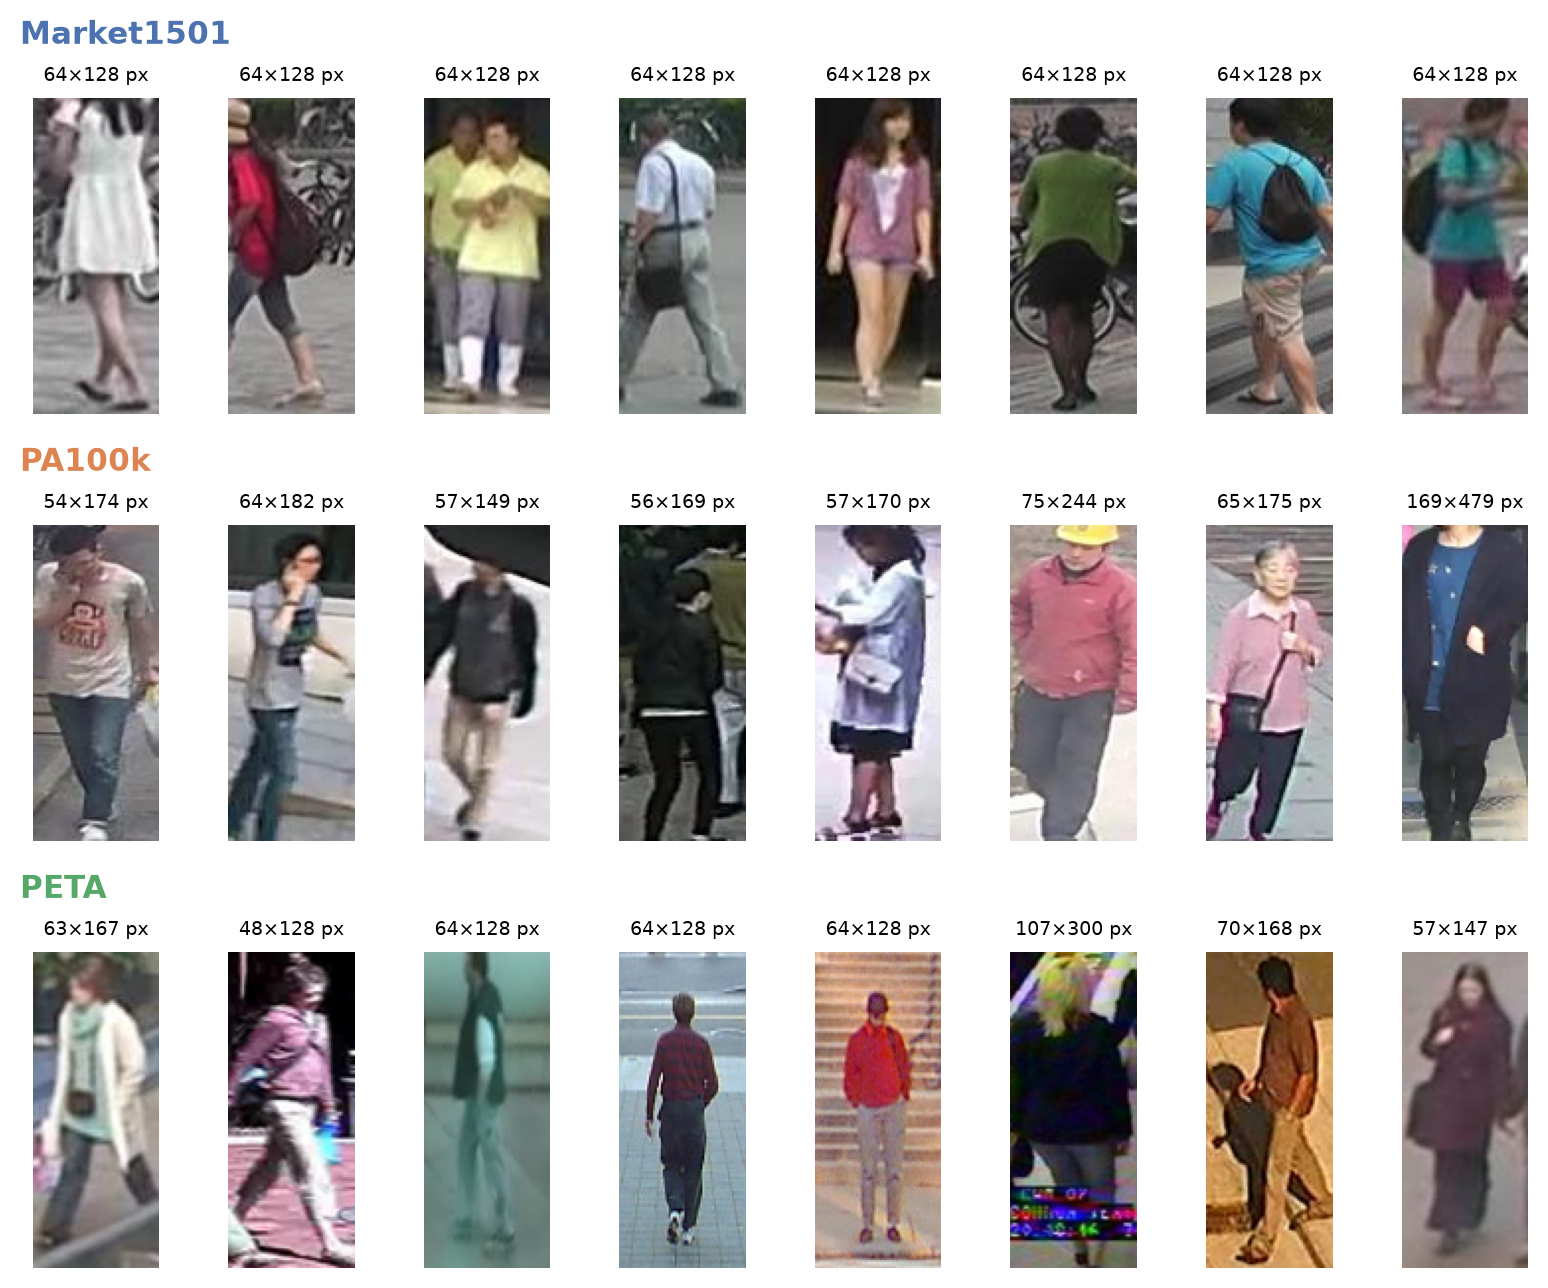
\includegraphics[width=0.74\linewidth]{samples.png}
\caption{Ảnh mẫu của ba bộ dữ liệu, kích thước gốc ghi phía trên mỗi ảnh. Ba miền khác nhau về độ phân giải, góc chụp và cân bằng màu.}
\label{fig:samples}
\end{figure}

Bốn mươi thuộc tính chia thành các nhóm gồm tuổi (trẻ, trưởng thành, già), giới tính nữ, độ dài tóc (ngắn, dài, hói), áo ngắn tay, 12 màu áo, quần ngắn, 12 màu quần, kiểu quần (quần dài hoặc ngắn, váy), và 5 phụ kiện (ba lô, túi, kính thường, kính râm, mũ). Màu sắc chiếm 24 trong 40 thuộc tính. Phần lớn các nhóm có cấu trúc loại trừ, ví dụ mỗi người có đúng một độ tuổi và thường có đúng một màu áo. Tần suất dương rất lệch (Hình~\ref{fig:comp}). Tỉ lệ người già là 1\% ở Market1501 nhưng hơn 6\% ở PETA, và một số màu không bao giờ được gán nhãn ở Market1501.

\begin{figure}[H]
\centering
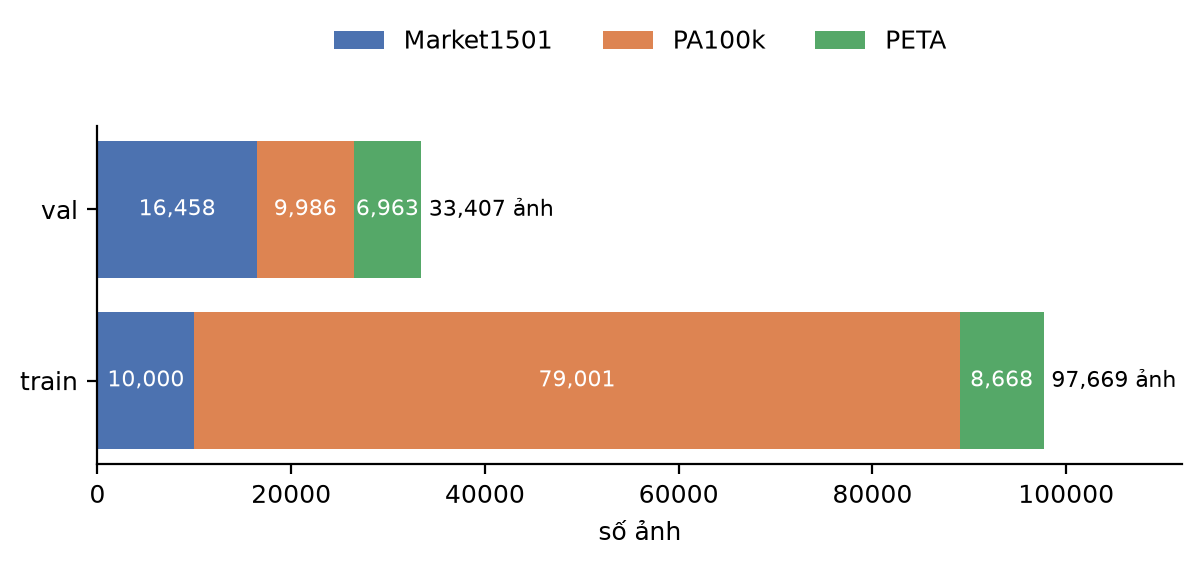
\includegraphics[width=0.92\linewidth]{composition.png}
\caption{Tần suất dương của các thuộc tính trong từng bộ dữ liệu. Tần suất khác nhau giữa các miền ở cùng một thuộc tính, đặc biệt ở tuổi và các màu hiếm, là nguồn gốc của dịch chuyển nhãn được phân tích ở mục~\ref{sec:thr}.}
\label{fig:comp}
\end{figure}

\subsection{Chỉ số đánh giá}
\label{sec:metric}

Tập chấm được đánh giá bằng hai họ chỉ số tính ở ngưỡng cố định 0.5, rồi gộp lại. Gọi $y_{ik}\in\{0,1\}$ là nhãn thật của ảnh $i$ ở thuộc tính $k$, và $\hat y_{ik}=\mathbb{1}[p_{ik}>0.5]$ là câu trả lời của chương trình.

Họ thứ nhất xét từng thuộc tính. \textbf{mA} (mean accuracy, tạm dịch: độ chính xác cân bằng trung bình) là trung bình của tỉ lệ dương được nhận ra và tỉ lệ âm được nhận ra, lấy trung bình trên 40 thuộc tính:
\begin{equation}
\mA=\frac{1}{K}\sum_{k=1}^{K}\frac12\left(\frac{\sum_i y_{ik}\hat y_{ik}}{\sum_i y_{ik}}+\frac{\sum_i (1-y_{ik})(1-\hat y_{ik})}{\sum_i (1-y_{ik})}\right).
\end{equation}
Mỗi thuộc tính có trọng số như nhau bất kể tần suất. Một chương trình luôn trả lời không cho thuộc tính ``người già'' đúng ở 99\% số ảnh Market1501, nhưng chỉ nhận 0.5 điểm cho thuộc tính này vì không nhận ra người già nào.

Họ thứ hai xét từng ảnh. Instance F1 so tập thuộc tính trả lời có với tập thuộc tính thật:
\begin{equation}
\IF=\frac{1}{N}\sum_{i=1}^{N}\frac{2\sum_k y_{ik}\hat y_{ik}}{\sum_k y_{ik}+\sum_k \hat y_{ik}}.
\end{equation}
Mỗi người có trung bình khoảng 7 thuộc tính dương trên 40, nên một câu trả lời có bị sai làm F1 của ảnh đó giảm từ 1 xuống khoảng 0.93. Điểm xếp hạng là trung bình điều hoà của hai họ, $\Avg = 2\,\mA\,\IF/(\mA+\IF)$.

Hai họ chỉ số kéo quyết định về hai phía ngược nhau. mA thưởng việc dám trả lời có ở thuộc tính hiếm, vì bỏ sót một mẫu dương hiếm bị phạt theo tỉ lệ nghịch với số mẫu dương. Instance F1 phạt mỗi câu trả lời có bị sai, bất kể thuộc tính hiếm hay phổ biến. Vì ngưỡng 0.5 cố định và không được điều chỉnh bởi bên chấm, vị trí ngưỡng hiệu dụng phải được mã hoá vào chính xác suất mà chương trình trả về. Hình~\ref{fig:tradeoff} minh hoạ đánh đổi này khi dời ngưỡng của mọi thuộc tính theo một hệ số chung.

\begin{figure}[H]
\centering
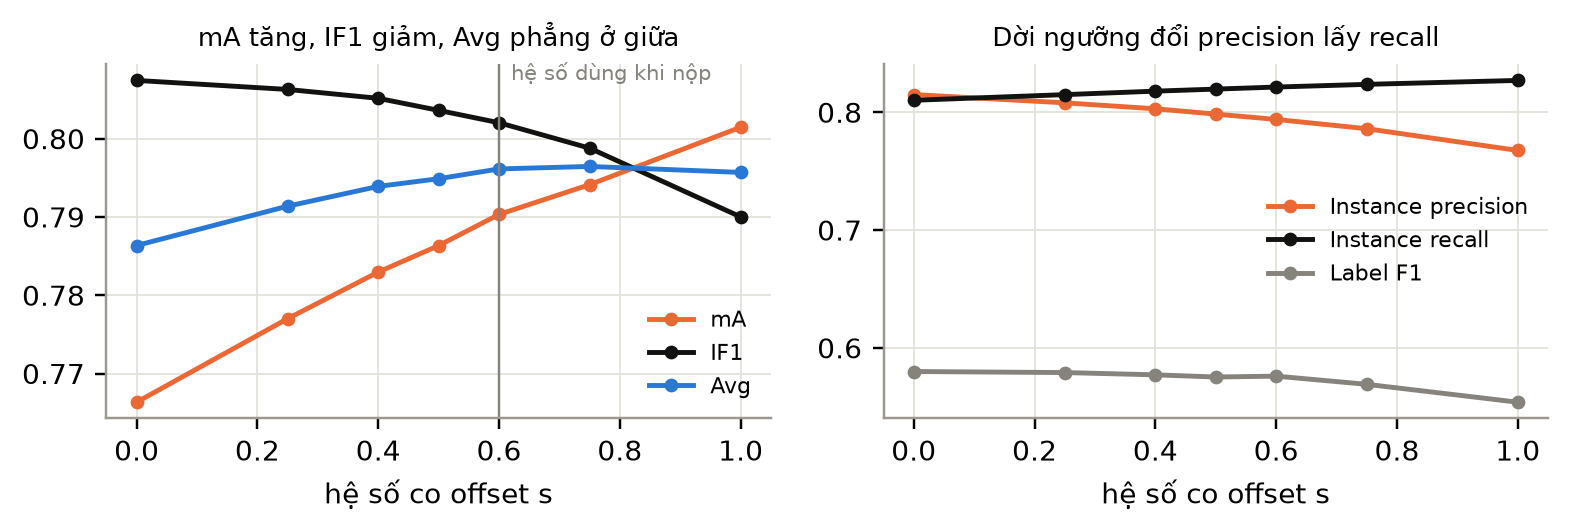
\includegraphics[width=0.95\linewidth]{v2_metric_tradeoff.png}
\caption{Dời ngưỡng theo hệ số $s$ của offset khớp trên miền nguồn, đo trên PETA giấu khỏi huấn luyện. mA tăng và Instance F1 giảm khi $s$ tăng, nên Avg tăng nhanh rồi gần như phẳng. Dời ngưỡng chỉ chọn vị trí trên đường đánh đổi, không đẩy được cả hai chỉ số cùng tăng.}
\label{fig:tradeoff}
\end{figure}

\subsection{Ràng buộc vận hành}
\label{sec:runtime}

Bài nộp là một gói mã nguồn. Chương trình chấm gọi hàm dự đoán trên 29.248 ảnh trong một container không có mạng, với 6 luồng CPU và giới hạn 3600 giây cho toàn bộ pha suy luận. Mỗi ngày được nộp ba lần. Bảng xếp hạng hiển thị bài nộp gần nhất chứ không phải bài tốt nhất. Môi trường chấm có PyTorch 2.4.1 và không có trình biên dịch C, nên không dùng được \texttt{torch.compile}. Hai hệ quả trực tiếp là thời gian chạy trở thành một siêu tham số ngang hàng với độ chính xác, và mọi lần nộp thất bại đều làm mất điểm hiển thị cho tới lần nộp kế tiếp.

\begin{ghichu}
Chỉ số Avg là một thoả hiệp giữa hai mục tiêu ngược nhau ở ngưỡng cố định 0.5. Vì vậy chất lượng của một hệ thống PAR trên miền mới có hai thành phần tách biệt được, gồm khả năng xếp hạng ảnh dương trên ảnh âm và vị trí ngưỡng. Hai thành phần này phản ứng khác nhau với dịch chuyển miền, và cần được đo riêng.
\end{ghichu}

%=====================================================================
\section{Nghiên cứu liên quan}
\label{sec:related}

\paragraph{Nhận dạng thuộc tính người đi bộ.} DeepMAR~\cite{deepmar} xây dựng PAR như phân loại đa nhãn với một backbone dùng chung và hàm mất mát entropy chéo nhị phân có trọng số theo tần suất. Các công trình sau tập trung vào việc định vị vùng ảnh liên quan tới từng thuộc tính, qua attention theo thuộc tính, mô-đun định vị theo thuộc tính, hoặc mô hình hoá quan hệ giữa thuộc tính. Jia và cộng sự~\cite{rethinkpar} chỉ ra rằng nhiều cải tiến được báo cáo biến mất khi ảnh của cùng một người không được xuất hiện ở cả train lẫn test, và một baseline đơn giản với backbone mạnh cạnh tranh được với các kiến trúc phức tạp. Kết quả của chúng tôi ở mục~\ref{sec:sweep} nhất quán với quan sát đó trong bối cảnh khác miền. Các head dựa trên truy vấn như Query2Label~\cite{q2l} và ML-Decoder~\cite{mldecoder} dùng một vector truy vấn học được cho mỗi nhãn và cross-attention lên các token ảnh. Chúng tôi dùng dạng head này.

\paragraph{UPAR và tổng quát hoá miền.} UPAR~\cite{upar} hợp nhất nhãn của PA100k, PETA, Market1501 và RAPv2 về 40 thuộc tính và đề xuất các giao thức huấn luyện trên một số miền, kiểm tra trên miền còn lại. Các báo cáo cuộc thi 2023 và 2024~\cite{upar23,upar24} ghi nhận rằng phần lớn đội thi khó vượt baseline trên miền mới, và việc cho phép huấn luyện trên nhiều miền giúp mô hình lớn tổng quát hoá tốt hơn. Trong tài liệu tổng quát hoá miền, Gulrajani và Lopez-Paz~\cite{domainbed} cho thấy khi so sánh công bằng, ERM với kiến trúc và dữ liệu tốt thường ngang hoặc hơn các thuật toán chuyên biệt, và việc chọn mô hình phải dựa trên miền giấu chứ không dựa trên miền nguồn. Chúng tôi áp dụng nguyên tắc chọn mô hình này.

\paragraph{Mô hình nền tảng thị giác.} DINOv2 và DINOv3~\cite{dinov3} học đặc trưng tự giám sát trên hàng tỉ ảnh và cho đặc trưng mạnh ở cả mức ảnh lẫn mức vùng. CLIP~\cite{clip} và các biến thể như MetaCLIP 2~\cite{metaclip2}, SigLIP 2~\cite{siglip2}, Perception Encoder~\cite{pe} học từ cặp ảnh và văn bản, nên đặc trưng của chúng gắn với khái niệm ngôn ngữ như tên màu và tên đồ vật. Các mô hình tổng hợp như AM-RADIO~\cite{radio} chưng cất nhiều mô hình nền tảng vào một mạng.

\paragraph{Chưng cất kiến thức.} Hinton và cộng sự~\cite{hinton} đề xuất huấn luyện mô hình trò khớp xác suất mềm của mô hình thầy. Beyer và cộng sự~\cite{patient} chỉ ra rằng chưng cất hiệu quả nhất khi thầy và trò nhìn cùng một ảnh đã tăng cường, kể cả ảnh trộn bằng mixup~\cite{mixup} hoặc CutMix~\cite{cutmix}, và khi huấn luyện đủ lâu. Họ gọi cách làm này là function matching. Chúng tôi dùng ý tưởng này ở mục~\ref{sec:kdmix}.

\paragraph{Dịch chuyển nhãn và điều chỉnh logit.} Khi phân bố tiên nghiệm của nhãn thay đổi giữa miền nguồn và miền đích nhưng phân bố ảnh theo nhãn giữ nguyên, xác suất hậu nghiệm có thể được hiệu chỉnh bằng tỉ số tiên nghiệm~\cite{saerens,lipton}. Menon và cộng sự~\cite{logitadj} dùng phép cộng logarit tỉ số tiên nghiệm vào logit để tối ưu độ chính xác cân bằng, chính là đại lượng mà mA đo. Mục~\ref{sec:thr} dẫn ra một biến thể của phép điều chỉnh này cho đúng hàm mất mát có trọng số mà chúng tôi dùng.

%=====================================================================
\section{Giao thức thẩm định khi không có tập chấm}
\label{sec:proxy}

\subsection{Vì sao điểm cùng miền không dùng được}

Chúng tôi không thấy ảnh của tập chấm và chỉ được nộp ba lần một ngày. Vì vậy mọi quyết định thiết kế phải dựa trên một phép đo cục bộ. Phép đo tự nhiên nhất là điểm trên tập val của chính ba bộ dữ liệu huấn luyện. Phép đo này không dùng được. Hệ thống đầu tiên của chúng tôi đạt 0.885 trên val cùng miền nhưng chỉ đạt 0.777 trên tập chấm. Khoảng cách 0.108 lớn hơn mọi khác biệt giữa các biến thể mà chúng tôi muốn so sánh, và thứ tự giữa các biến thể trên val cùng miền không khớp với thứ tự trên tập chấm.

\subsection{Giấu từng bộ dữ liệu}

Giao thức thay thế phải mô phỏng đúng điều kiện của tập chấm, gồm huấn luyện trên một số miền và kiểm tra trên một miền chưa thấy. Chúng tôi dùng \textbf{leave-one-dataset-out} (LODO, tạm dịch: giấu một bộ dữ liệu). Mô hình chỉ học từ train của hai bộ dữ liệu, rồi được chấm trên val của bộ thứ ba. Phiên bản chính giấu PETA, vì PETA gộp mười nguồn ảnh nhỏ và có thói quen gán nhãn khác hai bộ còn lại, nên là miền khó nhất. Hai phiên bản phụ giấu Market1501 và PA100k được dùng để kiểm tra một kết luận có lặp lại ở miền khác hay không.

Ngưỡng trong giao thức được xử lý giống hệt bài nộp. Offset của từng thuộc tính chỉ được khớp trên val của hai miền nhìn thấy, rồi áp lên miền giấu. Chúng tôi chấm checkpoint cuối cùng thay vì checkpoint tốt nhất theo miền giấu, vì chọn checkpoint theo chính miền giấu sẽ làm điểm lạc quan.

\subsection{Nhiễu và ngưỡng chấp nhận}

Hai lần chạy giống hệt nhau của cùng cấu hình ViT-B cho Avg 0.7961 và 0.7956 sau dời ngưỡng, nhưng lệch 0.0016 trước dời ngưỡng và 0.0033 ở AUC. Ngoài ra, khi chọn biến thể tốt nhất trong khoảng 35 biến thể có nhiễu độ lệch chuẩn $\sigma\approx0.001$, điểm của biến thể thắng bị thổi lên khoảng $2\sigma$. Vì hai lý do này, chúng tôi chỉ chấp nhận một thay đổi khi nó hơn mốc ít nhất 0.003 trên PETA giấu và không làm giảm điểm ở các miền giấu khác.

\subsection{Phân rã lỗi thành xếp hạng và ngưỡng}
\label{sec:decomp}

Một mô hình có thể mất điểm trên miền mới vì hai lý do khác nhau về bản chất. Lý do thứ nhất là nó không phân biệt được ảnh, ví dụ cho người áo đỏ và người áo cam xác suất ``áo đỏ'' gần bằng nhau. Lý do thứ hai là nó xếp hạng đúng nhưng mọi xác suất của một thuộc tính bị lệch đều về một phía, khiến ngưỡng 0.5 nằm sai chỗ. Khả năng xếp hạng được đo bằng \textbf{AUC} (tạm dịch: diện tích dưới đường cong ROC). AUC bằng xác suất một ảnh dương ngẫu nhiên có điểm cao hơn một ảnh âm ngẫu nhiên, nên không phụ thuộc vào ngưỡng.

Để tách hai lý do, chúng tôi khớp offset trực tiếp trên nhãn của miền giấu, gọi là \textbf{oracle offset}. Offset này không dùng được khi nộp bài, nhưng hiệu giữa điểm với oracle offset và điểm với offset khớp trên miền nguồn chính là phần điểm mất do ngưỡng. Hình~\ref{fig:gap} cho thấy phần này khoảng 0.02 trên PETA và tập trung ở các thuộc tính màu áo và màu quần.

\begin{figure}[H]
\centering
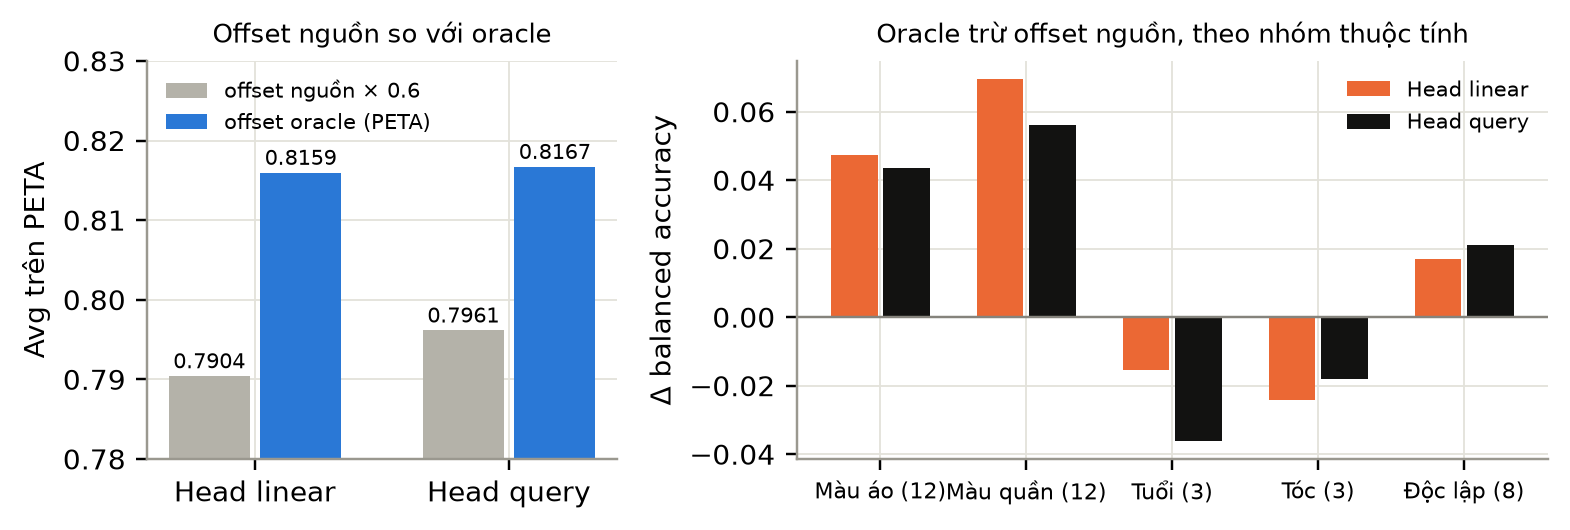
\includegraphics[width=\linewidth]{v2_gap.png}
\caption{Trái, điểm trên PETA giấu với offset khớp trên miền nguồn và với oracle offset. Khoảng cách khoảng 0.02 là phần điểm mất do vị trí ngưỡng. Phải, phần mất này tập trung ở hai nhóm màu.}
\label{fig:gap}
\end{figure}

Chúng tôi đã kiểm tra giả thuyết rằng lỗi ngưỡng ở nhóm màu do camera mới làm lệch cân bằng màu. Huấn luyện với tăng cường cân bằng trắng ngẫu nhiên không làm giảm phần lỗi này. Giải thích phù hợp hơn với dữ liệu là khác biệt trong quy ước gán nhãn màu. PETA đôi khi ghi hai màu cho một chiếc áo, không có nhãn ``màu khác'', trong khi hai bộ còn lại luôn ghi đúng một màu. Nếu giải thích này đúng, phần lỗi ngưỡng không thể sửa nếu không thấy nhãn của miền đích, và mọi tham số ngưỡng được tinh chỉnh trên PETA có nguy cơ chỉ khớp quy ước của PETA.

\subsection{Độ tin cậy của giao thức}
\label{sec:proxytest}

Hình~\ref{fig:pt} đối chiếu điểm thẩm định với điểm chấm thật của các bài nộp có cả hai số. Đổi backbone từ ViT-B sang ViT-L làm cả hai cùng tăng. Hai thay đổi chủ yếu tác động lên ngưỡng (head truy vấn trên ViT-B, và hệ số offset 1.0 thay cho 0.6) tăng trên giao thức thẩm định nhưng giảm trên tập chấm. Mức giảm của chúng (0.0025 và 0.0009) cùng cỡ với độ lệch giữa hai lần huấn luyện cùng cấu hình trên tập chấm (0.0019), nên bằng chứng chỉ ở mức gợi ý.

\begin{figure}[H]
\centering
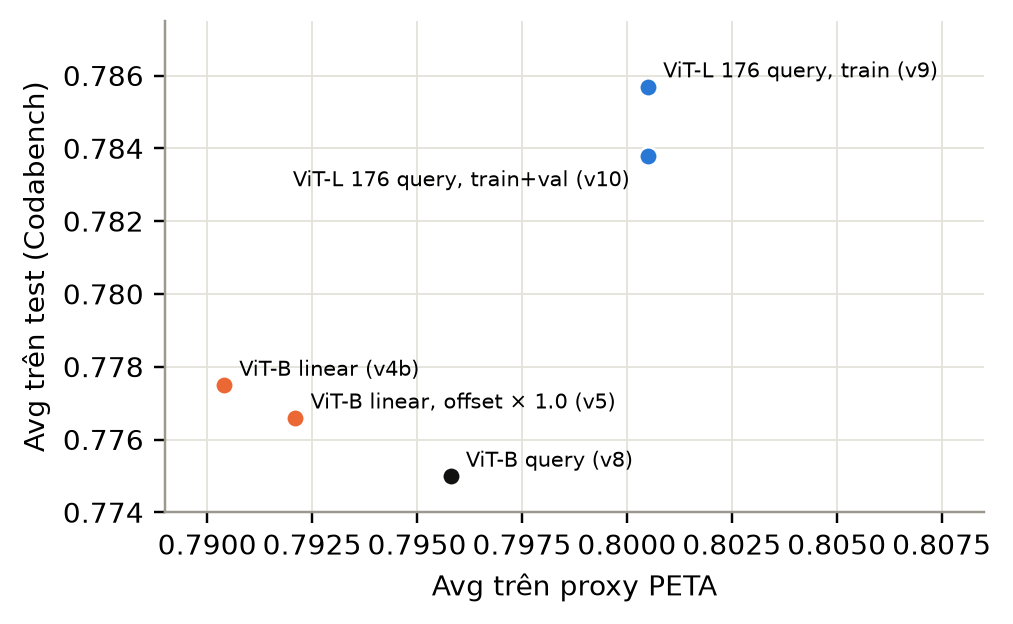
\includegraphics[width=0.5\linewidth]{v2_proxy_test.png}
\caption{Điểm thẩm định trên PETA giấu (trục ngang) so với điểm trên tập chấm ẩn (trục dọc). Thay đổi làm tăng AUC (đổi sang ViT-L) chuyển được sang tập chấm. Hai thay đổi tác động chủ yếu lên ngưỡng thì không.}
\label{fig:pt}
\end{figure}

\begin{ghichu}
Giao thức giấu một bộ dữ liệu đáng tin nhất với những thay đổi làm tăng khả năng xếp hạng (AUC). Một thay đổi chỉ làm tăng điểm thẩm định mà không tăng AUC nhiều khả năng chỉ khớp ngưỡng với quy ước gán nhãn của miền giấu, và cần bằng chứng từ ít nhất một miền giấu thứ hai trước khi được chấp nhận.
\end{ghichu}

%=====================================================================
\section{Phương pháp}
\label{sec:method}

\subsection{Tổng quan}

Hình~\ref{fig:pipeline} tóm tắt hệ thống. Khi suy luận, ảnh được đưa về kích thước cố định, đi qua backbone ViT để thành một dãy token, rồi một head truy vấn biến các token thành 40 logit. Mỗi logit được cộng một offset cố định theo quy tắc ở mục~\ref{sec:thr} trước khi qua hàm sigmoid. Khi huấn luyện, mô hình trò học đồng thời từ nhãn thật và từ logit trung bình của hai mô hình thầy lớn hơn.

\begin{figure}[H]
\centering
\begin{tikzpicture}[font=\sffamily\scriptsize, node distance=4mm and 5mm,
  box/.style={draw=black!55, rounded corners=2pt, fill=white, align=center, minimum height=8mm, inner sep=3pt},
  hl/.style={box, fill=acc!10, draw=acc!80!black},
  tc/.style={box, fill=org!10, draw=org!80!black},
  arr/.style={-{Latex[length=2mm]}, black!65}]
\node[box] (img) {Ảnh người\\ đi bộ};
\node[box, right=of img] (rs) {Resize\\176×96};
\node[hl, right=of rs] (bb) {DINOv3 ViT-L/16\\ 66 token ảnh\\ + token CLS};
\node[hl, right=of bb] (qh) {Head truy vấn\\ 40 truy vấn,\\ cross-attention};
\node[box, right=of qh] (lg) {40 logit\\ $z_k$};
\node[hl, right=of lg] (th) {$z_k + \tau\,b_k$\\ (mục~\ref{sec:thr})};
\node[box, right=of th] (pr) {40 xác suất\\ $\sigma(\cdot)$};
\draw[arr] (img)--(rs); \draw[arr] (rs)--(bb); \draw[arr] (bb)--(qh); \draw[arr] (qh)--(lg); \draw[arr] (lg)--(th); \draw[arr] (th)--(pr);
\node[tc, below=8mm of rs, xshift=6mm] (t1) {Thầy 1: DINOv3-L, 176×96, head truy vấn};
\node[tc, below=2mm of t1] (t2) {Thầy 2: CLIP-L/14, 168×84, head truy vấn};
\node[tc, right=8mm of $(t1.east)!0.5!(t2.east)$] (avg) {Trung bình\\ logit thầy $\bar z^{T}$};
\node[box, right=of avg, fill=black!3] (loss) {$\mathcal{L}=(1-\alpha)\mathcal{L}_{\text{nhãn}}$\\$+\,\alpha\,\mathcal{L}_{\text{KD}}(z,\bar z^{T})$};
\draw[arr] (t1.east) -- (avg.west |- t1.east); \draw[arr] (t2.east) -- (avg.west |- t2.east); \draw[arr] (avg)--(loss);
\draw[arr, dashed] (lg.south) |- ($(loss.north)+(0,3mm)$) -- (loss.north);
\node[font=\sffamily\scriptsize\itshape, text=black!55, anchor=west] at ($(t2.south west)+(0,-3mm)$) {chỉ dùng khi huấn luyện};
\end{tikzpicture}
\caption{Hệ thống nộp bài cuối (v13). Hàng trên là đường suy luận chạy trên CPU của máy chấm. Hàng dưới chỉ tồn tại khi huấn luyện. Hai mô hình thầy nhìn cùng ảnh đã tăng cường ở độ phân giải riêng, và logit trung bình của chúng làm mục tiêu mềm cho mô hình trò.}
\label{fig:pipeline}
\end{figure}

\subsection{Backbone}
\label{sec:backbone}

\paragraph{Vấn đề.} Mọi thông tin mà các tầng sau dùng tới đều phải có sẵn trong đặc trưng của backbone. Ở miền mới, backbone còn phải mã hoá màu, hình dạng và phụ kiện theo cách không phụ thuộc vào đặc điểm riêng của camera.

\paragraph{Lựa chọn.} Chúng tôi dùng DINOv3~\cite{dinov3}, tiền huấn luyện tự giám sát trên khoảng 1,7 tỉ ảnh, với kiến trúc ViT~\cite{vit}. ViT chia ảnh thành các \textbf{patch} (tạm dịch: mảnh ảnh) 16×16 pixel và biến mỗi patch thành một token. Chi phí tính toán tỉ lệ gần tuyến tính với số token ở các kích thước ảnh nhỏ này. Với ViT-B (86 triệu tham số), ảnh 256×128 cho 128 token và chạy khoảng 49,5 ms một ảnh trên máy chấm. ViT-L (khoảng 300 triệu tham số) chính xác hơn rõ rệt nhưng ở cùng kích thước ảnh cần khoảng 180 ms một ảnh, vượt ngân sách 123 ms.

\paragraph{Đánh đổi độ phân giải.} Cách duy nhất giữ được ViT-L trong ngân sách mà không mất độ chính xác do lượng tử hoá (mục~\ref{sec:neg}) là giảm số token. Bảng~\ref{tab:res} so các điểm làm việc. ViT-L ở 176×96 (66 token) cần 78 đến 98 ms một ảnh theo ước lượng và vẫn hơn ViT-B ở 256×128 khoảng 0.005 trên giao thức thẩm định. ViT-L ở 160×80 (50 token) đã kém ViT-B, cho thấy tồn tại một độ phân giải tối thiểu mà dưới đó backbone lớn mất lợi thế.

\begin{table}[H]
\centering\small
\begin{tabular}{@{}lcccc@{}}
\toprule
Backbone & Kích thước ảnh & Số token & ms/ảnh ước lượng trên máy chấm & Avg PETA giấu (offset × 0.6) \\
\midrule
ViT-B/16 & 256×128 & 128 & 49,5 (đo được) & 0.7958 \\
ViT-L/16 & 160×80 & 50 & không đo & 0.7891 \\
ViT-L/16 & 176×96 & 66 & 78 đến 98 & 0.8005 \\
ViT-L/16 & 192×96 & 72 & khoảng 95 & 0.8014 \\
ViT-L/16 & 224×112 & 98 & 118 đến 149 & 0.8071 \\
ViT-L/16 & 256×128 & 128 & khoảng 180 & không chạy \\
\bottomrule
\end{tabular}
\caption{Các điểm làm việc giữa độ chính xác và thời gian. Thời gian ước lượng bằng cách đo trong container giống máy chấm trên máy cá nhân, rồi quy đổi theo tỉ lệ đo được từ log của một bài nộp thật. Hai cách quy đổi cho hai giá trị khác nhau, nên một số dòng ghi khoảng. ViT-L 176×96 là cấu hình lớn nhất còn chừa biên an toàn so với ngân sách 123 ms theo cả hai cách quy đổi.}
\label{tab:res}
\end{table}

\begin{figure}[H]
\centering
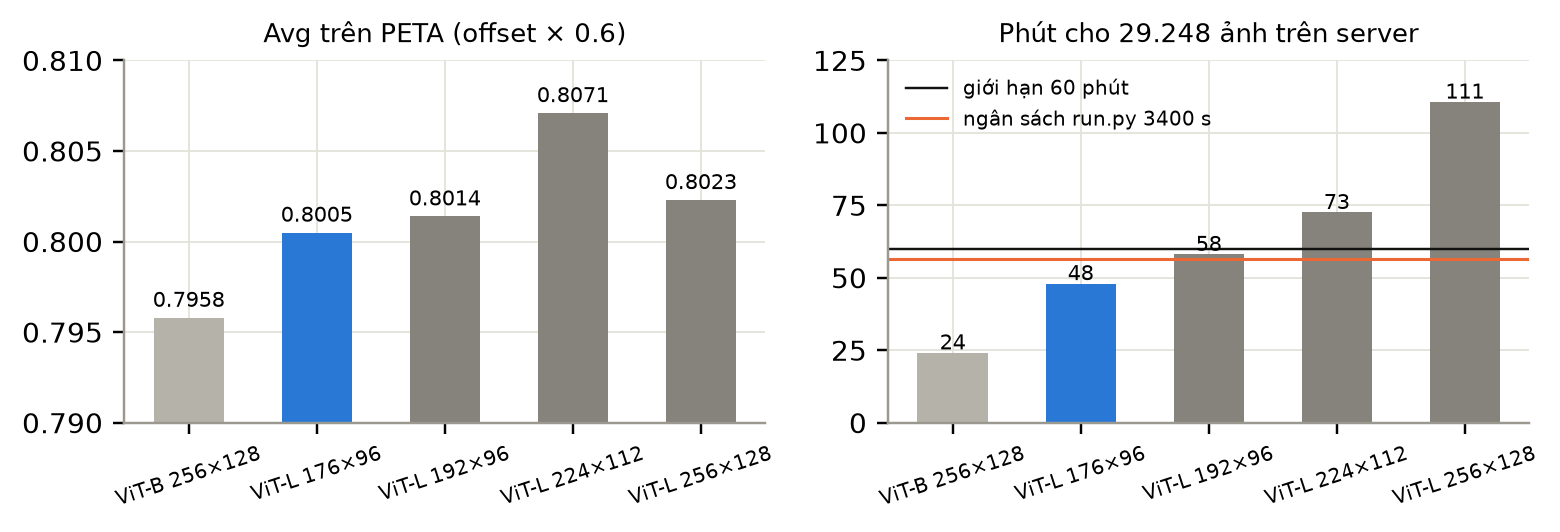
\includegraphics[width=\linewidth]{v2_vitl.png}
\caption{Trái, điểm thẩm định của ViT-B và ViT-L ở nhiều độ phân giải. Phải, thời gian ước lượng cho toàn bộ tập chấm so với giới hạn 60 phút. ViT-L 224×112 có điểm cao nhất nhưng vượt giới hạn, nên cấu hình 176×96 được chọn.}
\label{fig:vitl}
\end{figure}

\subsection{Head truy vấn theo thuộc tính}
\label{sec:head}

\paragraph{Vấn đề và khoảng trống.} Head tuyến tính lấy trung bình mọi token thành một vector chung rồi dự đoán cả 40 thuộc tính từ vector đó. Thuộc tính ``đội mũ'' vì thế phải dùng cùng một vector với thuộc tính ``màu quần'', dù hai thông tin nằm ở hai vùng ảnh khác nhau.

\paragraph{Cơ chế.} Head truy vấn gán cho mỗi thuộc tính $k$ một vector truy vấn học được $q_k\in\mathbb{R}^d$. Gọi $X\in\mathbb{R}^{n\times d}$ là ma trận gồm token CLS và $n-1$ token patch của backbone. Head tính
\begin{equation}
h_k = q_k + \mathrm{MHA}\big(\mathrm{LN}(q_k), \mathrm{LN}(X), \mathrm{LN}(X)\big), \qquad h'_k = h_k + \mathrm{MLP}(\mathrm{LN}(h_k)), \qquad z_k = w_k^\top \mathrm{LN}(h'_k) + c_k ,
\end{equation}
với LN là layer normalization, MHA là multi-head attention 8 đầu, MLP có hệ số mở rộng 2, và $w_k, c_k$ là bộ phân loại riêng của thuộc tính $k$. Trong MHA, trọng số attention của truy vấn $k$ lên token $j$ tỉ lệ với $\exp(q_k^\top W_Q^\top W_K x_j/\sqrt{d_h})$. Truy vấn của thuộc tính ``mũ'' vì thế học cách gán trọng số cao cho các token ở vùng đầu. Head có một tầng và chiếm dưới 0,1\% số phép tính của backbone, nên không ảnh hưởng tới ngân sách thời gian.

\subsection{Hàm mất mát}
\label{sec:loss}

Hàm mất mát nhãn là entropy chéo nhị phân với hai điều chỉnh. Thứ nhất, nhãn được làm mềm với hệ số $\epsilon=0.05$. Nhãn 1 trở thành 0.975 và nhãn 0 trở thành 0.025. Điều chỉnh này giới hạn mức phạt khi nhãn gốc sai, vốn xảy ra thường xuyên với thuộc tính màu. Thứ hai, mỗi ô được nhân trọng số kiểu DeepMAR~\cite{deepmar}, $w^+_k=e^{1-p_k}$ cho ô dương và $w^-_k=e^{p_k}$ cho ô âm, với $p_k$ là tần suất dương của thuộc tính $k$ trên tập train. Tỉ số $w^+_k/w^-_k=e^{1-2p_k}$ không vượt quá $e$, nên thuộc tính hiếm được ưu tiên vừa phải.
\begin{equation}
\mathcal{L}_{\text{nhãn}} = -\frac{1}{|\mathcal{V}|}\sum_{(i,k)\in\mathcal{V}} \Big[w^+_k\,\tilde y_{ik}\log\sigma(z_{ik}) + w^-_k(1-\tilde y_{ik})\log(1-\sigma(z_{ik}))\Big].
\end{equation}
Tập $\mathcal{V}$ chỉ gồm các ô có nhãn. Market1501 không gán nhãn một số thuộc tính, và các ô đó không đóng góp vào loss.

Các bộ dữ liệu được lấy mẫu theo xác suất tỉ lệ với $N_d^{0.5}$, với $N_d$ là số ảnh của bộ $d$. Với tập train, cách lấy mẫu này giảm tỉ trọng của PA100k từ 81\% xuống khoảng 59\% số ảnh mỗi epoch ($\sqrt{79001}$ so với $\sqrt{79001}+\sqrt{10000}+\sqrt{8668}$), mà không lặp lại ảnh của hai bộ nhỏ quá nhiều lần.

\subsection{Chưng cất từ nhiều thầy}
\label{sec:kd}

\paragraph{Vấn đề.} ViT-L ở 176×96 là mô hình lớn nhất vừa ngân sách, nhưng các mô hình lớn hơn hoặc chạy ở độ phân giải cao hơn cho điểm tốt hơn và không thể nộp. Ngoài ra, các mô hình tiền huấn luyện theo kiểu khác DINOv3, như CLIP, có thể mã hoá thông tin mà DINOv3 thiếu.

\paragraph{Thuộc tính cần có.} Phương pháp cần chuyển được lợi ích của các mô hình không nộp được sang mô hình nộp được, mà không thay đổi chi phí suy luận.

\paragraph{Ý tưởng cốt lõi.} Một tổ hợp các mô hình có lỗi ít tương quan xếp hạng tốt hơn từng thành viên. Huấn luyện mô hình trò khớp logit của tổ hợp cho trò một tín hiệu học phong phú hơn nhãn cứng, vì logit của thầy mã hoá cả mức độ chắc chắn và các tương quan giữa thuộc tính.

\paragraph{Cơ chế.} Mỗi thầy là một mô hình đầy đủ (backbone và head truy vấn) được tinh chỉnh 3 epoch trên cùng dữ liệu, đóng băng 8 block đầu. Thầy 1 là DINOv3-L ở 176×96, thầy 2 là CLIP-L/14~\cite{clip} ở 168×84. Khi huấn luyện trò, mỗi batch ảnh đã tăng cường được đưa qua từng thầy ở độ phân giải và chuẩn hoá màu riêng của thầy đó. Logit của các thầy được lấy trung bình thành $\bar z^{T}$. Loss chưng cất là entropy chéo nhị phân giữa xác suất của trò và xác suất của thầy ở nhiệt độ $T$:
\begin{equation}
\mathcal{L}_{\text{KD}} = T^2\cdot\frac{1}{NK}\sum_{i,k}\mathrm{BCE}\Big(\sigma(z_{ik}/T),\ \sigma(\bar z^{T}_{ik}/T)\Big), \qquad \mathcal{L}=(1-\alpha)\,\mathcal{L}_{\text{nhãn}}+\alpha\,\mathcal{L}_{\text{KD}} .
\end{equation}
Hệ số $T^2$ giữ độ lớn gradient không phụ thuộc vào nhiệt độ~\cite{hinton}. Khác với loss nhãn, loss chưng cất tính trên mọi ô, kể cả các ô không có nhãn ở Market1501, vì thầy cung cấp được mục tiêu cho cả những ô đó. Cấu hình nộp dùng $\alpha=0.8$, $T=1$ và 10 epoch.

\subsubsection{Function matching với ảnh trộn}
\label{sec:kdmix}

Theo Beyer và cộng sự~\cite{patient}, chưng cất hiệu quả hơn khi trò được hỏi về những ảnh nằm ngoài phân bố ảnh huấn luyện, để nó học khớp hàm của thầy chứ không chỉ khớp nhãn. Với xác suất 0.5, chúng tôi thay batch bằng một batch trộn, nửa số lần bằng mixup ($\lambda\sim\mathrm{Beta}(0.8,0.8)$) và nửa số lần bằng CutMix ($\lambda\sim\mathrm{Beta}(1,1)$). Nhãn thật không mô tả được ảnh trộn, nên batch trộn chỉ dùng loss chưng cất. Biến thể này cần huấn luyện lâu hơn (20 epoch) và được dùng cho các bài nộp ViT-B ở cả Track 1 và Track 2.

\subsection{Quy tắc dời ngưỡng theo dịch chuyển nhãn}
\label{sec:thr}

\paragraph{Vấn đề.} Ngưỡng 0.5 cố định, nên vị trí quyết định hiệu dụng phải được mã hoá vào xác suất trả về. Cách làm truyền thống là khớp một offset $o_k$ cho từng thuộc tính bằng tìm kiếm lưới, tối đa hoá Avg trên val của miền nguồn, rồi nhân với một hệ số $s<1$ để bớt khớp quá mức.

\paragraph{Khoảng trống.} Offset khớp trên miền nguồn mang theo cả tần suất nhãn lẫn quy ước gán nhãn của miền nguồn. Mục~\ref{sec:decomp} đã cho thấy phần lỗi ngưỡng trên miền mới đến chủ yếu từ quy ước gán nhãn. Offset khớp trên dữ liệu vì vậy dễ khớp nhầm thông tin không chuyển được sang miền đích. Ngoài ra hệ số $s$ được chọn bằng chính giao thức thẩm định, tạo ra vòng lặp chọn tham số.

\paragraph{Thuộc tính cần có.} Quy tắc cần dời ngưỡng theo hướng mà chỉ số đánh giá ưu tiên, nhưng chỉ dùng những đại lượng ít phụ thuộc vào quy ước gán nhãn, như tần suất dương trung bình.

\paragraph{Ý tưởng cốt lõi.} Nếu mô hình được hiệu chỉnh đúng theo tiên nghiệm $p_k$ của tập train, xác suất hậu nghiệm của nó là $P(y=1\mid x)$ dưới tiên nghiệm $p_k$. Độ chính xác cân bằng, đại lượng mà mA đo, là độ chính xác dưới tiên nghiệm cân bằng $0.5$. Theo phép hiệu chỉnh tiên nghiệm~\cite{saerens,logitadj}, chuyển từ tiên nghiệm $p_k$ sang tiên nghiệm 0.5 tương đương cộng vào logit một lượng $\log\frac{1-p_k}{p_k}$. Tuy nhiên trọng số DeepMAR trong loss đã dời logit tối ưu một lượng $\log(w^+_k/w^-_k) = 1-2p_k$ theo cùng hướng. Phần còn thiếu để đạt quyết định cân bằng là
\begin{equation}
b_k = \log\frac{1-p_k}{p_k} - (1-2p_k).
\label{eq:theory}
\end{equation}
Instance F1 lại ưu tiên quyết định không cân bằng, vì mỗi câu trả lời có bị sai đều làm giảm F1. Vì vậy chúng tôi chỉ đi một phần quãng đường, với offset cuối là $\tau b_k$ và $\tau\in[0,1]$. Giá trị $\tau=0$ giữ nguyên quyết định của loss có trọng số, còn $\tau=1$ là quyết định tối ưu cho mA.

\paragraph{Tính chất.} Quy tắc~\eqref{eq:theory} chỉ dùng tần suất dương $p_k$ trên toàn bộ dữ liệu huấn luyện, không dùng điểm của bất kỳ miền nào, và có một tham số chung $\tau$ cho cả 40 thuộc tính thay vì 40 offset. Với thuộc tính hiếm như ``người già'' ($p\approx0.03$), $b_k\approx 3.48-0.94=2.54$, nên ngưỡng hiệu dụng giảm mạnh. Với thuộc tính phổ biến như ``quần dài'' ($p\approx0.8$), $b_k\approx -1.39+0.60=-0.79$, nên ngưỡng hiệu dụng tăng nhẹ. Chúng tôi chọn $\tau=0.42$ trên các lần chạy giấu PETA. Lựa chọn này có cùng vòng lặp chọn tham số như hệ số $s$, nhưng chỉ với một tham số thay vì 40 offset cộng một hệ số.

\subsection{Triển khai trên CPU}
\label{sec:deploy}

Mô hình được xuất thành TorchScript đã đóng băng, chạy fp32 trên 6 luồng với batch 32 đến 64 ảnh. Chúng tôi đo từng thành phần của thời gian chạy. Đọc và tiền xử lý ảnh mất khoảng 0,4 ms một ảnh, còn backbone chiếm gần toàn bộ phần còn lại. Đóng băng TorchScript nhanh hơn khoảng 3\%, chia batch thành khối 32 ảnh nhanh hơn khoảng 7\%. bf16 chỉ có lợi trên CPU có lệnh \texttt{amx\_bf16} hoặc \texttt{avx512\_bf16}. Trên CPU không có các lệnh này, bf16 được giả lập và chậm hơn khoảng 60 lần, nên chương trình kiểm tra cờ CPU trước khi chọn kiểu số.

Các bài nộp đầu có một cơ chế dự phòng. Nếu đến phút thứ 57 chương trình chưa xong, các ảnh còn lại nhận xác suất trung bình. Mục~\ref{sec:lb} cho thấy cơ chế này gây hại nhiều hơn có lợi, và các bài nộp sau bỏ nó.

\begin{ghichu}
Trong bài toán này, mỗi thành phần của hệ thống được chọn bằng hai phép đo độc lập, gồm điểm trên miền giấu và thời gian trên máy chấm. Thời gian không phải ràng buộc phụ áp dụng sau cùng. Nó quyết định kích thước backbone và độ phân giải, và hai yếu tố này chi phối độ chính xác nhiều hơn mọi lựa chọn kiến trúc khác.
\end{ghichu}

%=====================================================================
\section{Thực nghiệm}
\label{sec:exp}

\subsection{Thiết lập}

Mọi mô hình được tinh chỉnh với AdamW, learning rate $5\cdot10^{-5}$ ở block cuối và giảm theo hệ số 0.75 cho mỗi block về phía đầu vào (layer decay), learning rate của head gấp 10 lần, weight decay 0.05, warmup 0,5 epoch, lịch cosine, batch 64, và trung bình động mũ của trọng số với hệ số 0.9995. Tăng cường dữ liệu gồm lật ngang, đệm 10 pixel rồi cắt ngẫu nhiên, giảm độ phân giải ngẫu nhiên với xác suất 0.3 để mô phỏng ảnh chụp xa, và thay đổi độ sáng, độ tương phản. Không đổi tông màu, vì màu là nhãn. Các lần chạy thẩm định ViT-B dùng 5 epoch. Huấn luyện chạy trên GPU thuê (RTX 5090 và A100 80 GB).

\subsection{Khảo sát head, loss và tăng cường dữ liệu}
\label{sec:sweep}

Với backbone ViT-B cố định, chúng tôi thử khoảng 35 thay đổi chia thành bốn nhóm. Nhóm kiến trúc head gồm head tuyến tính, head truy vấn 1 và 2 tầng, head kép, đọc token từ 4 tầng cuối, MixStyle~\cite{mixstyle}, MoE trên token, quét tuần tự kiểu Mamba, attention tuần tự theo nhóm, decoder 4 tầng, CNN, bộ phân loại riêng theo bộ dữ liệu, và head có tiên nghiệm không gian. Nhóm loss và cách huấn luyện gồm LP-FT~\cite{lpft}, ASL~\cite{asl}, logit adjustment~\cite{logitadj}, entropy chéo theo nhóm, cân bằng bộ dữ liệu, che nhãn nhiễu và các decoder tái tạo phụ trợ. Nhóm dữ liệu gồm tăng cường mạnh, cân bằng trắng ngẫu nhiên và lọc nhãn. Nhóm backbone gồm PE-Core~\cite{pe}, SigLIP 2~\cite{siglip2}, EUPE, TIPSv2, C-RADIOv3~\cite{radio} và ViT-L ở nhiều độ phân giải.

\begin{figure}[H]
\centering
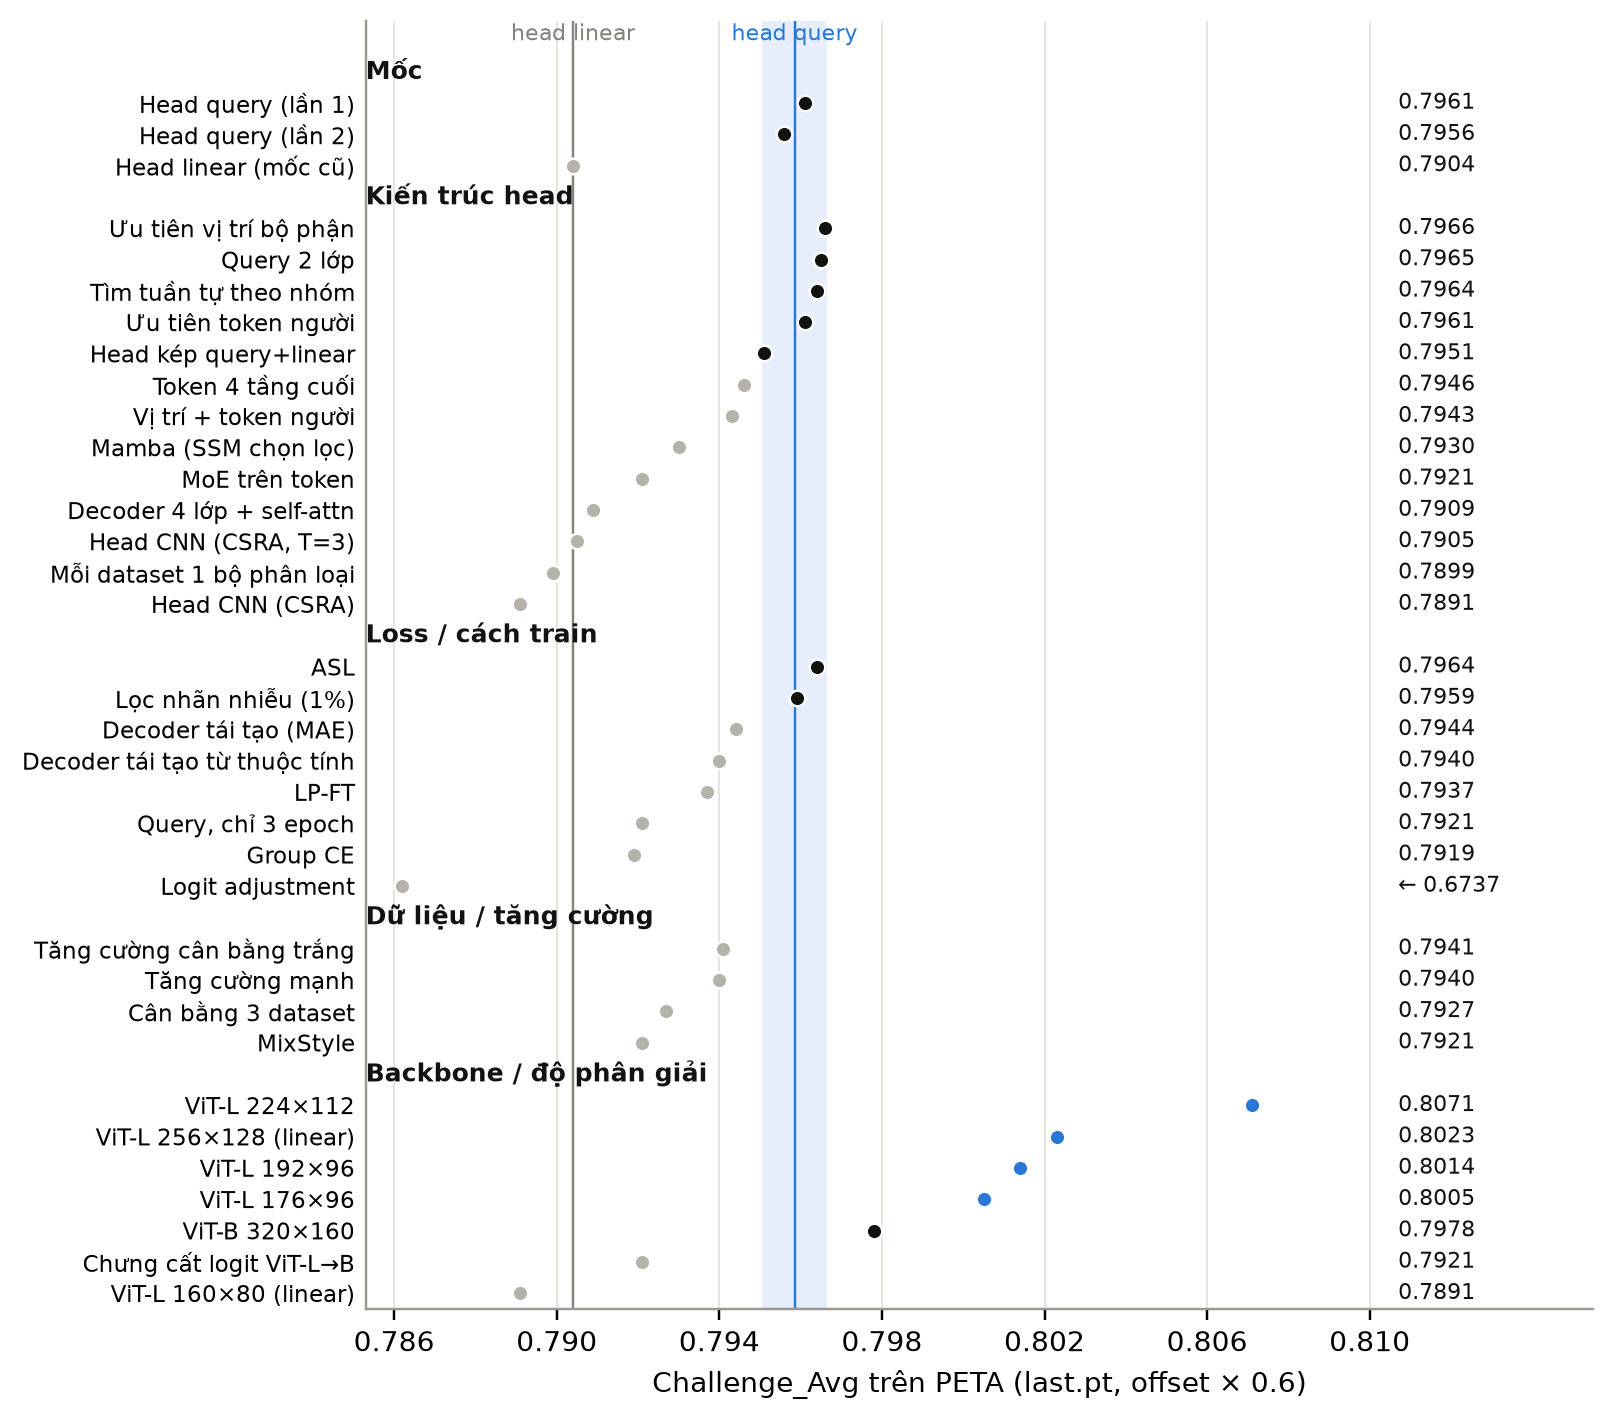
\includegraphics[width=0.84\linewidth]{v2_experiments.png}
\caption{Điểm thẩm định trên PETA giấu của khoảng 35 thay đổi. Dải xanh là mốc head truy vấn cộng trừ mức dao động giữa hai lần chạy. Chỉ các thay đổi backbone sang ViT-L (điểm xanh) vượt mốc quá ngưỡng chấp nhận 0.003.}
\label{fig:sweep}
\end{figure}

Hình~\ref{fig:sweep} cho thấy mọi thay đổi ở head, loss và tăng cường dữ liệu nằm quanh mốc hoặc thấp hơn. AUC của mọi biến thể ViT-B nằm trong khoảng 0.898 đến 0.908, trong khi ViT-L đạt 0.910 đến 0.913. Cách giải thích đơn giản nhất là mọi head đọc cùng một bộ đặc trưng. Nếu bộ đặc trưng không đủ thông tin để xếp hạng hai ảnh, không phép biến đổi nào ở head tạo ra được thông tin đó. Các thay đổi loss như ASL hay logit adjustment chủ yếu dời ngưỡng, và mục~\ref{sec:decomp} đã cho thấy phần điểm do ngưỡng không chuyển ổn định sang miền mới. Các backbone thay thế đều kém DINOv3 ở cùng kích thước, kể cả các mô hình tổng hợp nhiều thầy như C-RADIOv3-B (0.7757 trên tập chấm so với 0.7775 của DINOv3-B).

\subsection{Tính bổ trợ giữa các mô hình thầy}
\label{sec:comp}

\paragraph{Câu hỏi.} Cần chọn mô hình ghép với DINOv3-L làm thầy. Một giả thuyết tự nhiên là ghép với mô hình mạnh nhất. Giả thuyết cạnh tranh là ghép với mô hình khác DINOv3 nhất, vì lợi ích của tổ hợp đến từ các lỗi không tương quan.

\paragraph{Thiết kế.} Chúng tôi tinh chỉnh 11 mô hình nền tảng cỡ L hoặc lớn hơn trên giao thức giấu PETA với cùng công thức (3 epoch, đóng băng 8 block, head truy vấn), rồi lấy trung bình logit của DINOv3-L với từng mô hình và chấm trên PETA. Độ tương quan giữa hai mô hình được đo bằng trung bình hệ số tương quan Pearson giữa logit của chúng trên từng thuộc tính.

\begin{figure}[H]
\centering
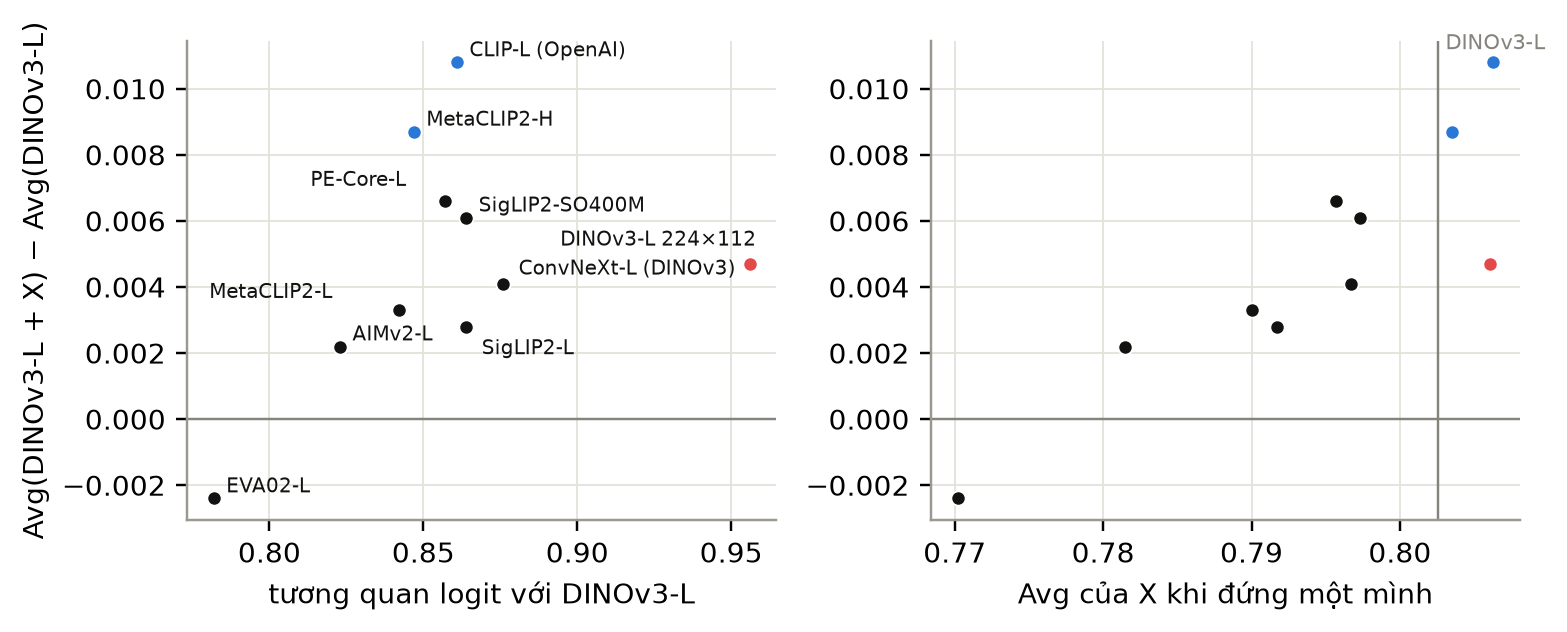
\includegraphics[width=\linewidth]{complementarity.png}
\caption{Lợi ích khi ghép DINOv3-L với từng mô hình X, chấm trên PETA giấu. Trái, lợi ích theo độ tương quan logit với DINOv3-L. Phải, lợi ích theo điểm của X khi đứng một mình. Hai mô hình học từ cặp ảnh và văn bản (xanh) cho lợi ích lớn nhất. Một bản DINOv3-L khác độ phân giải (đỏ) mạnh ngang CLIP-L khi đứng một mình nhưng cho lợi ích chưa bằng một nửa, vì tương quan quá cao (0.956).}
\label{fig:comp2}
\end{figure}

\paragraph{Kết quả.} Hình~\ref{fig:comp2} hỗ trợ giả thuyết thứ hai. DINOv3-L ở 224×112 có điểm riêng 0.8061, gần bằng CLIP-L (0.8063), nhưng khi ghép với DINOv3-L 176×96 chỉ tăng 0.0047, so với 0.0108 của CLIP-L. Tương quan logit của nó với DINOv3-L là 0.956, cao hơn hẳn mọi mô hình khác (0.78 đến 0.88). Trong nhóm có tương quan thấp, điểm riêng lẻ quyết định lợi ích. EVA02-L có tương quan thấp nhất nhưng điểm riêng chỉ 0.7702, và ghép với nó còn làm giảm điểm. Hai mô hình học từ cặp ảnh và văn bản là CLIP-L và MetaCLIP2-H~\cite{metaclip2} đứng đầu. Ghép cả ba (DINOv3-L, CLIP-L, MetaCLIP2-H) đạt 0.8137 sau dời ngưỡng và 0.8168 với quy tắc lý thuyết, AUC 0.9248, cao nhất trong mọi tổ hợp chúng tôi đo (Bảng~\ref{tab:ens}).

\begin{table}[H]
\centering\small
\begin{tabular}{@{}lccc@{}}
\toprule
Tổ hợp logit (PETA giấu) & Avg, offset × 0.6 & Avg, $\tau=0.42$ & AUC \\
\midrule
DINOv3-L một mình & 0.8026 & 0.8078 & 0.9126 \\
DINOv3-L + CLIP-L & 0.8134 & 0.8146 & 0.9203 \\
DINOv3-L + MetaCLIP2-H & 0.8113 & 0.8149 & 0.9239 \\
DINOv3-L + CLIP-L + MetaCLIP2-H & 0.8137 & 0.8168 & 0.9248 \\
DINOv3-L + CLIP-L + PE-Core-L & 0.8118 & 0.8139 & 0.9223 \\
DINOv3-L + CLIP-L + SigLIP2-SO400M & 0.8101 & 0.8153 & 0.9233 \\
\midrule
DINOv3-L + CLIP-L, trọng số riêng từng thuộc tính & 0.8120 & 0.8148 & 0.9192 \\
3 thầy, trọng số riêng từng thuộc tính & 0.8127 & 0.8167 & 0.9214 \\
\bottomrule
\end{tabular}
\caption{Tổ hợp logit của các thầy trên PETA giấu. Trọng số riêng cho từng thuộc tính, khớp trên val của miền nguồn, không hơn trung bình đều. Điều này nhất quán với kết luận ở mục~\ref{sec:decomp} rằng tham số khớp trên miền nguồn ít chuyển được sang miền mới.}
\label{tab:ens}
\end{table}

Chúng tôi cũng thử thay trung bình đều bằng trọng số riêng cho từng thuộc tính, khớp trên val của miền nguồn theo log-loss. Ý tưởng là thuộc tính màu có thể nên tin CLIP nhiều hơn, còn thuộc tính dáng người nên tin DINOv3 nhiều hơn. Cách này không cải thiện (hai dòng cuối của Bảng~\ref{tab:ens}). Các trọng số học được phản ánh mô hình nào giỏi thuộc tính nào trên miền nguồn, và quan hệ đó thay đổi trên miền mới.

\subsection{Chưng cất chuyển được bao nhiêu}
\label{sec:transfer}

Tổ hợp hai thầy hơn DINOv3-L một mình 0.0108. Câu hỏi thực tế là mô hình trò, vốn có kích thước và độ phân giải của DINOv3-L 176×96, giữ được bao nhiêu phần lợi đó. Hình~\ref{fig:transfer} trả lời câu hỏi này cho hai cỡ trò.

\begin{figure}[H]
\centering
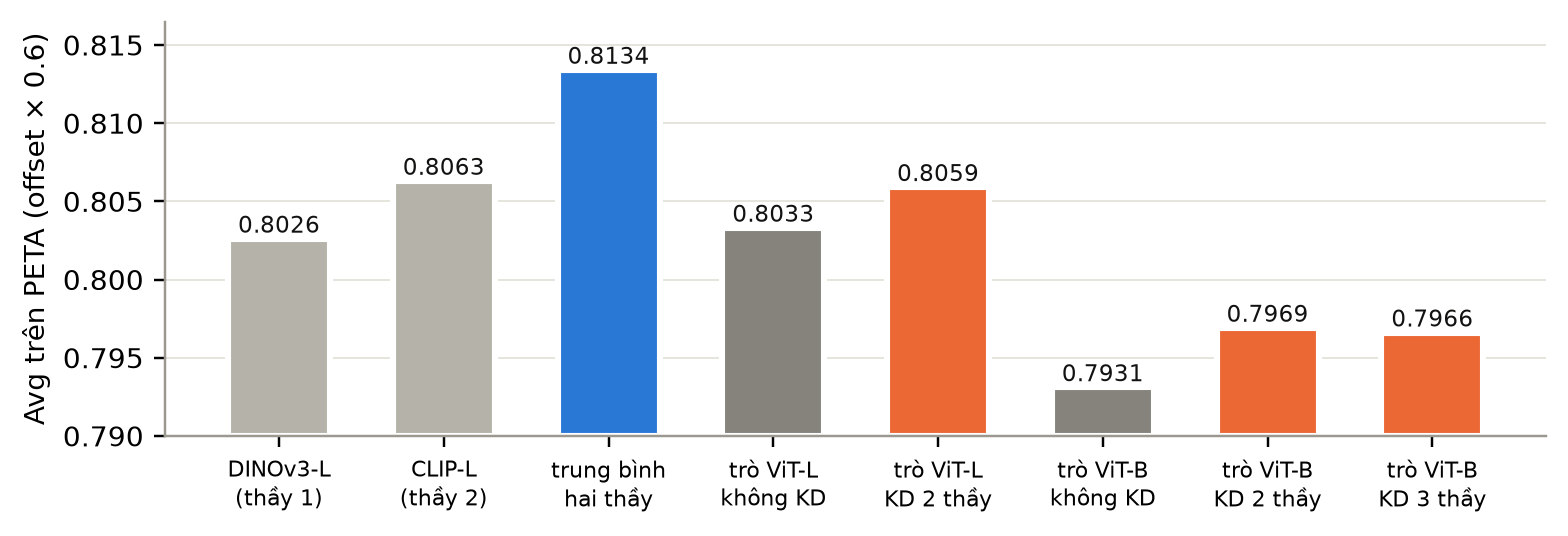
\includegraphics[width=\linewidth]{transfer.png}
\caption{Lợi ích của tổ hợp thầy và phần chuyển được sang trò, trên PETA giấu. Trò ViT-L giữ được 0.0026 trong 0.0108 điểm lợi của tổ hợp. Trò ViT-B tăng 0.0038 so với ViT-B không chưng cất, và thêm thầy thứ ba không cải thiện trò ViT-B.}
\label{fig:transfer}
\end{figure}

Trò ViT-L học từ hai thầy đạt 0.8059, so với 0.8033 khi không chưng cất. Như vậy trò giữ được khoảng một phần tư lợi ích của tổ hợp. Chúng tôi cần lưu ý rằng một lần chạy ViT-L không chưng cất với lịch 3 epoch đạt 0.8072. Do đó mức tăng của chưng cất trên Avg nằm trong biên độ dao động giữa các lịch huấn luyện. Thứ tăng ổn định là AUC, từ 0.907 đến 0.913 lên 0.920 đến 0.923 ở mọi cấu hình chưng cất (Bảng~\ref{tab:kd}).

\begin{table}[H]
\centering\small
\begin{tabular}{@{}llcccc@{}}
\toprule
Trò & Thầy, cấu hình & Avg × 0.6 & Avg $\tau$ 0.42 & AUC & mADM (Track 2) \\
\midrule
ViT-L 176 & không chưng cất, 5 epoch & 0.8033 & & 0.9071 & 0.6496 \\
ViT-L 176 & không chưng cất, 3 epoch & 0.8072 & & 0.9128 & 0.6531 \\
ViT-L 176 & DINOv3-L + CLIP-L, $\alpha$ 0.8, 6 epoch & 0.8059 & 0.8098 & 0.9205 & 0.6635 \\
ViT-L 176 & DINOv3-L + CLIP-L, $\alpha$ 0.8, 10 epoch & 0.8057 & & 0.9222 & 0.6681 \\
ViT-L 176 & DINOv3-L + MetaCLIP2-H, 10 epoch & 0.8061 & & 0.9233 & 0.6697 \\
ViT-L 176 & 3 thầy (+ DINOv3-L 224), 6 epoch & 0.8038 & 0.8077 & 0.9194 & 0.6590 \\
ViT-L 176 & DINOv3-L + CLIP-L, kd-mix, 20 epoch & 0.8064 & 0.8122 & 0.9230 & 0.6751 \\
\midrule
ViT-B 256 & không chưng cất & 0.7931 & & 0.8975 & 0.6406 \\
ViT-B 256 & DINOv3-L + CLIP-L, kd-mix, 10 epoch & 0.7969 & 0.8024 & 0.9155 & 0.6577 \\
ViT-B 256 & 3 thầy (+ MetaCLIP2-H), kd-mix, 10 epoch & 0.7966 & 0.8012 & 0.9165 & 0.6582 \\
\bottomrule
\end{tabular}
\caption{Chưng cất trên PETA giấu. Chưng cất làm AUC tăng ổn định 0.007 đến 0.019, nhưng Avg sau dời ngưỡng chỉ tăng trong biên độ dao động. Thầy thứ ba giống DINOv3 (DINOv3-L 224) làm trò kém đi, còn thầy thứ ba khác kiểu (MetaCLIP2-H) không thay đổi trò ViT-B.}
\label{tab:kd}
\end{table}

Ba quan sát rút ra từ Bảng~\ref{tab:kd}. Thứ nhất, thầy thứ ba chỉ có ích nếu nó bổ trợ. DINOv3-L 224 làm trò ViT-L kém đi 0.002, vì nó kéo mục tiêu mềm về phía DINOv3 vốn đã là backbone của trò. Thứ hai, ngay cả thầy thứ ba bổ trợ (MetaCLIP2-H) cũng không cải thiện trò ViT-B, dù tổ hợp ba thầy hơn tổ hợp hai thầy 0.0022 với quy tắc lý thuyết. Giới hạn vì vậy nằm ở sức chứa của trò. Thứ ba, chưng cất có lợi lớn hơn rõ rệt cho Track 2 (mADM tăng 0.014 đến 0.026) so với Track 1. Track 2 xếp hạng bằng log-likelihood của cả vector xác suất, nên được hưởng trực tiếp xác suất có hiệu chỉnh tốt hơn mà thầy cung cấp, trong khi Avg chỉ nhìn ở một ngưỡng.

\subsection{Quy tắc ngưỡng}
\label{sec:threxp}

\begin{figure}[H]
\centering
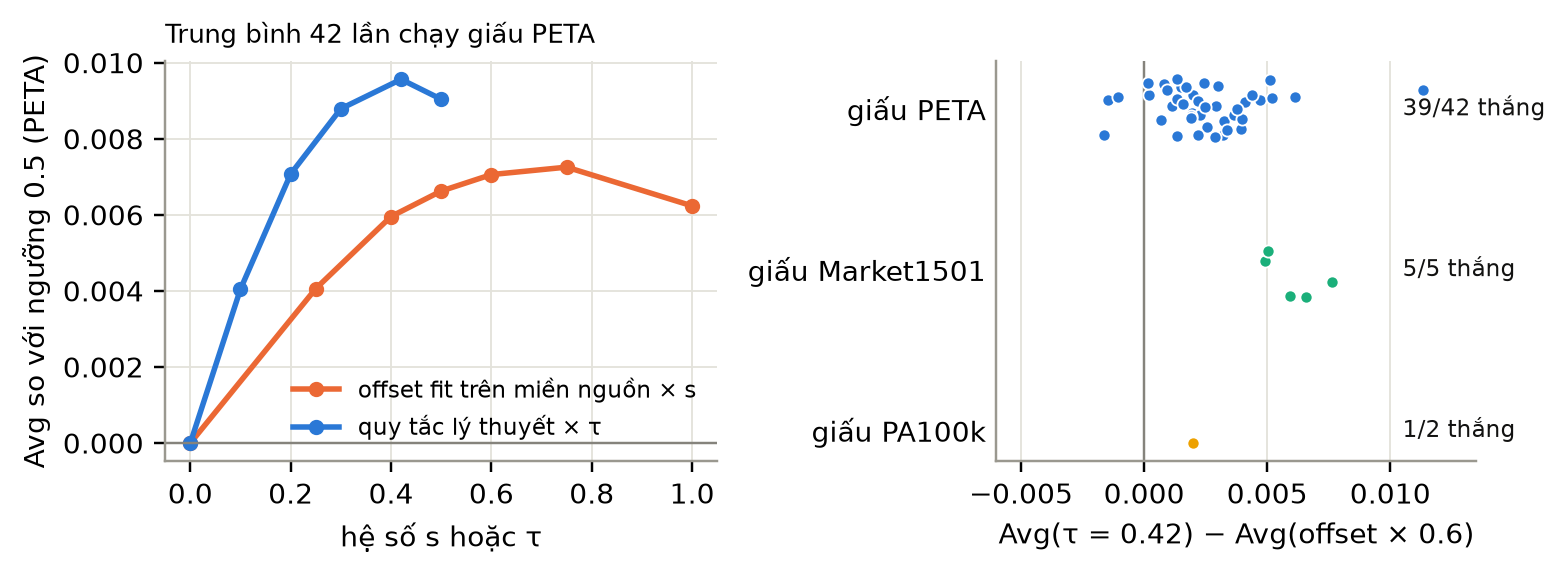
\includegraphics[width=\linewidth]{thresholds.png}
\caption{Trái, mức tăng Avg so với ngưỡng 0.5 của hai họ quy tắc, trung bình trên 42 lần chạy giấu PETA. Quy tắc lý thuyết đạt đỉnh cao hơn và sớm hơn. Phải, chênh lệch giữa quy tắc lý thuyết $\tau=0.42$ và offset khớp × 0.6 trên từng lần chạy. Quy tắc lý thuyết thắng ở 45 trên 49 lần chạy, gồm cả hai miền giấu không dùng để chọn $\tau$.}
\label{fig:thr}
\end{figure}

Hình~\ref{fig:thr} so hai họ quy tắc trên 49 lần chạy thẩm định với nhiều backbone, head và loss khác nhau. Trung bình trên các lần chạy giấu PETA, quy tắc lý thuyết đạt mức tăng 0.0096 ở $\tau=0.42$, so với 0.0073 của offset khớp ở hệ số tốt nhất ($s=0.75$) và 0.0071 ở hệ số đang dùng ($s=0.6$). Quan trọng hơn, quy tắc lý thuyết thắng ở cả 5 lần chạy giấu Market1501, vốn không tham gia việc chọn $\tau$. Trên tập chấm, áp quy tắc này lên đúng mô hình của bài nộp v12 nâng điểm từ 0.7896 lên 0.7912. Mức tăng 0.0016 nhỏ, nhưng cùng hướng với giao thức thẩm định và đạt được mà không thay đổi mô hình.

\subsection{Những gì không hiệu quả}
\label{sec:neg}

Bảng~\ref{tab:neg} tóm tắt các hướng đã thử và bị loại ngoài khảo sát ở mục~\ref{sec:sweep}. Chúng tôi ghi lại chúng vì hai lý do. Chúng giới hạn không gian tìm kiếm cho người làm tiếp, và một số trong đó là các kỹ thuật được khuyến nghị rộng rãi trong tài liệu.

\begin{table}[H]
\centering\small
\begin{tabularx}{\linewidth}{@{}p{4.3cm}X@{}}
\toprule
Hướng & Kết quả và lý do \\
\midrule
Lượng tử hoá int8 động & ViT-B val 0.885 xuống 0.703 khi lượng tử hoá mọi tầng, xuống 0.809 khi chỉ lượng tử hoá qkv và fc1. ViT-L trên PETA giấu giảm từ 0.809 xuống 0.765. Đặc trưng của DINOv3 có giá trị ngoại lai lớn ở một số kênh, nên lượng tử hoá theo tensor mất thông tin. \\
Model soup~\cite{soup} & Trung bình trọng số của các head huấn luyện với seed khác nhau làm điểm sụp xuống khoảng 0.75. Soup cùng khởi tạo chỉ ngang các thành phần trên PETA, và soup của v12 với một trò mới làm AUC trên val giảm. \\
Chưng cất logit ViT-L sang ViT-B, chỉ nhãn cứng & Tăng 0.0017 trên giao thức thẩm định nhưng bài nộp (KD-B) đạt 0.7717, thấp hơn ViT-B không chưng cất 0.0058. \\
Trọng số chưng cất theo độ đồng thuận của thầy & Không tăng so với trung bình đều. \\
Chuẩn hoá logit của thầy trước khi trung bình & Không tăng. \\
Backbone thay thế cỡ B & PE-Core, SigLIP 2, EUPE, TIPSv2, C-RADIOv3-B đều kém DINOv3-B sau tinh chỉnh. \\
Tăng cường cân bằng trắng & Không giảm lỗi ngưỡng ở nhóm màu, ủng hộ giả thuyết quy ước gán nhãn ở mục~\ref{sec:decomp}. \\
Thêm thầy thứ ba cho trò ViT-B & Ngang hai thầy (0.7966 so với 0.7969). \\
\bottomrule
\end{tabularx}
\caption{Các hướng đã thử và bị loại. Phần lớn các hướng hoặc không tăng khả năng xếp hạng, hoặc làm mất thông tin đặc trưng của backbone.}
\label{tab:neg}
\end{table}

%=====================================================================
\section{Kết quả trên tập chấm ẩn}
\label{sec:lb}

\subsection{Lịch sử bài nộp}

Hình~\ref{fig:lb} và Bảng~\ref{tab:lb} liệt kê các bài nộp theo thứ tự. Ba bước tạo ra phần lớn mức tăng. Đổi sang ViT-L 176×96 tăng 0.0082 (từ 0.7775 lên 0.7857). Chưng cất từ DINOv3-L và CLIP-L tăng thêm 0.0039 (lên 0.7896). Quy tắc ngưỡng lý thuyết tăng thêm 0.0016 (lên 0.7912). Mọi thay đổi khác trên ViT-B, kể cả head truy vấn, đều nằm trong khoảng $\pm0.003$ quanh 0.776.

\begin{figure}[H]
\centering
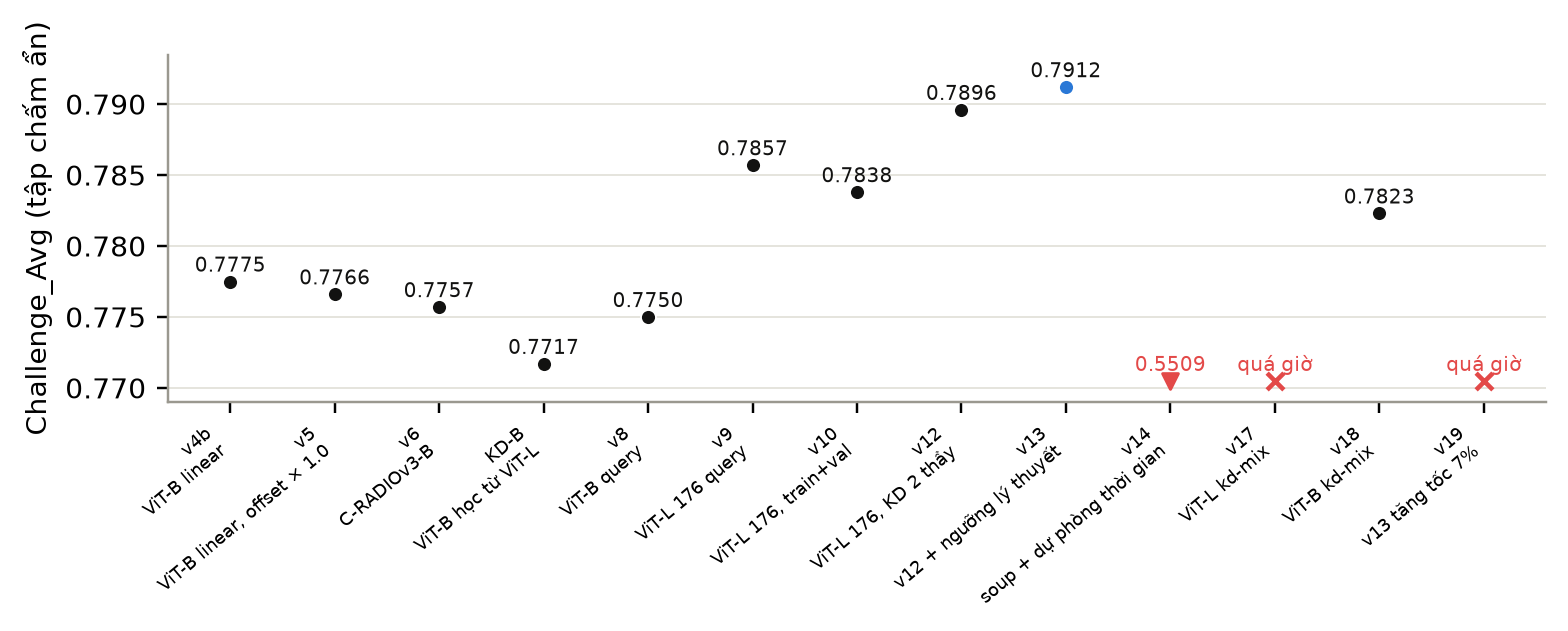
\includegraphics[width=\linewidth]{leaderboard.png}
\caption{Điểm trên tập chấm ẩn theo thứ tự nộp. Điểm xanh là bài tốt nhất (v13). Dấu tam giác đỏ là bài bị cơ chế dự phòng thời gian làm hỏng. Dấu chéo đỏ là bài không chạy xong trong thời gian cho phép.}
\label{fig:lb}
\end{figure}

\begin{table}[H]
\centering\small
\begin{tabularx}{\linewidth}{@{}llXc@{}}
\toprule
Bài & Backbone & Thay đổi chính & Tập chấm \\
\midrule
v4b & ViT-B 256 & head tuyến tính, train+val, offset × 0.6 & 0.7775 \\
v5 & ViT-B 256 & như v4b, offset × 1.0 & 0.7766 \\
v6 & C-RADIOv3-B & đổi backbone & 0.7757 \\
KD-B & ViT-B 256 & chưng cất logit từ ViT-L & 0.7717 \\
v8 & ViT-B 256 & head truy vấn & 0.7750 \\
v9 & ViT-L 176 & head truy vấn, train & 0.7857 \\
v10 & ViT-L 176 & như v9, train+val & 0.7838 \\
v12 & ViT-L 176 & chưng cất DINOv3-L + CLIP-L, train+val & 0.7896 \\
v13 & ViT-L 176 & v12 + quy tắc ngưỡng $\tau=0.42$ & 0.7912 \\
v14 & ViT-L 176 & soup + dự phòng thời gian & 0.5509 \\
v17 & ViT-L 176 & kd-mix 20 epoch, không dự phòng & không xong \\
v18 & ViT-B 256 & kd-mix 20 epoch, $\tau=0.42$ & 0.7823 \\
v19 & ViT-L 176 & mô hình v13, tối ưu tốc độ 7\% & không xong (2 giờ) \\
\bottomrule
\end{tabularx}
\caption{Các bài nộp Track 1 có ghi nhận kết quả. Bài v13 đứng đầu bảng xếp hạng tại thời điểm nộp. Sau v14, các bài ViT-L không còn chạy xong ổn định, nên bài hiển thị hiện tại là v18 dùng ViT-B.}
\label{tab:lb}
\end{table}

\subsection{Độ biến thiên tốc độ của máy chấm}

Ba bài nộp ViT-L sau v13 cho thấy một vấn đề mà giao thức thẩm định không đo được. Các log của Track 2, vốn dùng cùng môi trường chấm, ghi nhận ViT-L 176×96 chạy 103 ms một ảnh ở một lần và 176 đến 190 ms một ảnh ở các lần khác. Với 29.248 ảnh, 103 ms một ảnh cho khoảng 50 phút, còn 190 ms một ảnh cho khoảng 93 phút, vượt xa giới hạn 60 phút. Bài v13 chạy xong ở một lần máy nhanh. Bài v19 dùng đúng mô hình đó với một tối ưu tốc độ 7\%, nhưng không xong sau 2 giờ.

Cơ chế dự phòng của v14 làm tình huống tệ hơn. Khi máy chậm, chương trình trả về xác suất trung bình cho một phần lớn số ảnh, và bài nộp nhận 0.5509 thay vì thất bại. Vì bảng xếp hạng hiển thị bài gần nhất, điểm hiển thị giảm từ 0.7912 xuống 0.5509. Một bài thất bại thì không thay thế bài trước đó. Từ đó, chúng tôi bỏ mọi cơ chế dự phòng và thiết kế ngân sách theo máy chậm nhất đã quan sát. Với ràng buộc này, chỉ mô hình cỡ ViT-B còn an toàn, và bài v18 (ViT-B chưng cất kd-mix) đạt 0.7823.

\begin{ghichu}
Khi môi trường chấm có tốc độ dao động, một bài nộp chỉ đáng tin nếu nó chạy kịp ở lần chậm nhất đã quan sát. Cơ chế dự phòng trả về kết quả kém thay vì thất bại là có hại khi bảng xếp hạng hiển thị bài gần nhất, vì nó thay một điểm tốt bằng một điểm xấu.
\end{ghichu}

%=====================================================================
\section{Thảo luận}
\label{sec:disc}

\paragraph{Nút thắt là backbone, sau đó là bước chuyển giao.} Khảo sát ở mục~\ref{sec:sweep} cho thấy với backbone cố định, các lựa chọn ở head, loss và tăng cường dữ liệu không thay đổi khả năng xếp hạng vượt quá nhiễu. Mức tăng thật sự đến từ hai nguồn, gồm backbone lớn hơn (ViT-L) và tín hiệu từ các mô hình lớn hơn nữa qua chưng cất. Phân tích ở mục~\ref{sec:transfer} cho thấy bước chưng cất chỉ giữ khoảng một phần tư lợi ích của tổ hợp thầy, và trò ViT-B không hấp thụ thêm khi tổ hợp thầy mạnh hơn. Hướng đáng làm tiếp vì vậy là cải thiện bước chuyển giao, ví dụ chưng cất đặc trưng mức token thay vì chỉ logit, hoặc tăng lượng ảnh không nhãn mà trò được hỏi.

\paragraph{Thông tin chuyển được và thông tin không chuyển được.} Các phép đo nhất quán với một phân chia. Khả năng xếp hạng, đo bằng AUC, chuyển được từ miền nguồn sang miền mới. Vị trí ngưỡng tối ưu, gắn với quy ước gán nhãn của từng miền, thì không. Ba kết quả độc lập ủng hộ phân chia này, gồm việc proxy đoán sai đúng hai thay đổi kiểu ngưỡng, việc trọng số tổ hợp riêng theo thuộc tính không chuyển được, và việc quy tắc ngưỡng ít tham số thắng quy tắc khớp nhiều tham số. Chúng tôi coi đây là giả thuyết được hỗ trợ, chưa được chứng minh, vì chưa có phép đo trực tiếp nhãn của miền đích.

\paragraph{Giới hạn của báo cáo.} Mức nhiễu giữa các lần chạy chỉ được ước lượng từ vài cặp lần chạy lặp. Giá trị $\tau=0.42$ được chọn trên chính các lần chạy giấu PETA. Các thời gian ước lượng trên máy chấm dựa trên một số ít log, và chính các log này cho thấy tốc độ dao động gần hai lần. Cuối cùng, phần lớn kết luận dựa trên một miền giấu chính (PETA), với hai miền giấu phụ chỉ được dùng cho một số so sánh.

%=====================================================================
\section{Kết luận}

Chúng tôi trình bày một hệ thống PAR cho miền camera chưa thấy dưới ràng buộc chỉ dùng CPU, đạt 0.7912 Challenge\_Avg trên tập chấm ẩn của UPAR Challenge 2027 Track 1. Hệ thống kết hợp backbone DINOv3 ViT-L ở độ phân giải được chọn theo ngân sách thời gian, head truy vấn, chưng cất từ hai thầy có kiểu tiền huấn luyện bổ trợ, và quy tắc dời ngưỡng suy ra từ giả thiết dịch chuyển nhãn. Các thí nghiệm có kiểm soát cho thấy thứ quyết định kết quả là khả năng xếp hạng của đặc trưng, còn các tham số được khớp trên miền nguồn, dù là ngưỡng hay trọng số tổ hợp, ít chuyển được sang miền mới. Về vận hành, độ dao động tốc độ của máy chấm buộc hệ thống phải được thiết kế cho trường hợp chậm nhất, và cơ chế dự phòng trả về kết quả kém có hại hơn một lần chạy thất bại.

%=====================================================================
\begin{thebibliography}{99}\small
\bibitem{upar} A.~Specker, M.~Cormier, J.~Beyerer. UPAR: Unified pedestrian attribute recognition and person retrieval. \textit{WACV}, 2023.
\bibitem{upar23} M.~Cormier, A.~Specker, J.~C.~S.~Jacques Junior và cộng sự. UPAR challenge: Pedestrian attribute recognition and attribute-based person retrieval, dataset, design, and results. \textit{WACV Workshops}, 2023.
\bibitem{upar24} M.~Cormier, A.~Specker, J.~C.~S.~Jacques Junior và cộng sự. UPAR challenge 2024: Pedestrian attribute recognition and attribute-based person retrieval, dataset, design, and results. \textit{WACV Workshops}, 2024.
\bibitem{peta} Y.~Deng, P.~Luo, C.~C.~Loy, X.~Tang. Pedestrian attribute recognition at far distance. \textit{ACM Multimedia}, 2014.
\bibitem{pa100k} X.~Liu, H.~Zhao, M.~Tian và cộng sự. HydraPlus-Net: Attentive deep features for pedestrian analysis. \textit{ICCV}, 2017.
\bibitem{market} L.~Zheng, L.~Shen, L.~Tian và cộng sự. Scalable person re-identification: A benchmark. \textit{ICCV}, 2015.
\bibitem{marketattr} Y.~Lin, L.~Zheng, Z.~Zheng và cộng sự. Improving person re-identification by attribute and identity learning. \textit{Pattern Recognition}, 2019.
\bibitem{deepmar} D.~Li, X.~Chen, K.~Huang. Multi-attribute learning for pedestrian attribute recognition in surveillance scenarios. \textit{ACPR}, 2015.
\bibitem{rethinkpar} J.~Jia, H.~Huang, X.~Chen, K.~Huang. Rethinking of pedestrian attribute recognition: A reliable evaluation under zero-shot pedestrian identity setting. \textit{arXiv:2107.03576}, 2021.
\bibitem{q2l} S.~Liu, L.~Zhang, X.~Yang, H.~Su, J.~Zhu. Query2Label: A simple transformer way to multi-label classification. \textit{arXiv:2107.10834}, 2021.
\bibitem{mldecoder} T.~Ridnik, G.~Sharir, A.~Ben-Cohen, E.~Ben-Baruch, A.~Noy. ML-Decoder: Scalable and versatile classification head. \textit{WACV}, 2023.
\bibitem{domainbed} I.~Gulrajani, D.~Lopez-Paz. In search of lost domain generalization. \textit{ICLR}, 2021.
\bibitem{dinov3} O.~Siméoni, H.~V.~Vo, M.~Seitzer và cộng sự. DINOv3. \textit{arXiv:2508.10104}, 2025.
\bibitem{vit} A.~Dosovitskiy, L.~Beyer, A.~Kolesnikov và cộng sự. An image is worth 16x16 words: Transformers for image recognition at scale. \textit{ICLR}, 2021.
\bibitem{clip} A.~Radford, J.~W.~Kim, C.~Hallacy và cộng sự. Learning transferable visual models from natural language supervision. \textit{ICML}, 2021.
\bibitem{metaclip2} Y.-S.~Chuang và cộng sự. MetaCLIP 2: A worldwide scaling recipe. \textit{arXiv:2507.22062}, 2025.
\bibitem{siglip2} M.~Tschannen và cộng sự. SigLIP 2: Multilingual vision-language encoders with improved semantic understanding, localization, and dense features. \textit{arXiv:2502.14786}, 2025.
\bibitem{pe} D.~Bolya và cộng sự. Perception Encoder: The best visual embeddings are not at the output of the network. \textit{arXiv:2504.13181}, 2025.
\bibitem{radio} M.~Ranzinger, G.~Heinrich, J.~Kautz, P.~Molchanov. AM-RADIO: Agglomerative vision foundation model, reduce all domains into one. \textit{CVPR}, 2024.
\bibitem{hinton} G.~Hinton, O.~Vinyals, J.~Dean. Distilling the knowledge in a neural network. \textit{arXiv:1503.02531}, 2015.
\bibitem{patient} L.~Beyer, X.~Zhai, A.~Royer, L.~Markeeva, R.~Anil, A.~Kolesnikov. Knowledge distillation: A good teacher is patient and consistent. \textit{CVPR}, 2022.
\bibitem{mixup} H.~Zhang, M.~Cisse, Y.~N.~Dauphin, D.~Lopez-Paz. mixup: Beyond empirical risk minimization. \textit{ICLR}, 2018.
\bibitem{cutmix} S.~Yun, D.~Han, S.~J.~Oh và cộng sự. CutMix: Regularization strategy to train strong classifiers with localizable features. \textit{ICCV}, 2019.
\bibitem{saerens} M.~Saerens, P.~Latinne, C.~Decaestecker. Adjusting the outputs of a classifier to new a priori probabilities: A simple procedure. \textit{Neural Computation}, 2002.
\bibitem{lipton} Z.~C.~Lipton, Y.-X.~Wang, A.~Smola. Detecting and correcting for label shift with black box predictors. \textit{ICML}, 2018.
\bibitem{logitadj} A.~K.~Menon, S.~Jayasumana, A.~S.~Rawat và cộng sự. Long-tail learning via logit adjustment. \textit{ICLR}, 2021.
\bibitem{mixstyle} K.~Zhou, Y.~Yang, Y.~Qiao, T.~Xiang. Domain generalization with MixStyle. \textit{ICLR}, 2021.
\bibitem{lpft} A.~Kumar, A.~Raghunathan, R.~Jones, T.~Ma, P.~Liang. Fine-tuning can distort pretrained features and underperform out-of-distribution. \textit{ICLR}, 2022.
\bibitem{asl} T.~Ridnik, E.~Ben-Baruch, N.~Zamir và cộng sự. Asymmetric loss for multi-label classification. \textit{ICCV}, 2021.
\bibitem{soup} M.~Wortsman, G.~Ilharco, S.~Y.~Gadre và cộng sự. Model soups: Averaging weights of multiple fine-tuned models improves accuracy without increasing inference time. \textit{ICML}, 2022.
\end{thebibliography}

%=====================================================================
\appendix
\section{Siêu tham số chi tiết}
\label{app:hp}

\begin{table}[H]
\centering\small
\begin{tabularx}{\linewidth}{@{}lX@{}}
\toprule
Thành phần & Giá trị \\
\midrule
Backbone trò (v12, v13) & \texttt{vit\_large\_patch16\_dinov3.lvd1689m}, 176×96, chuẩn hoá ImageNet \\
Head & truy vấn, 1 tầng, 8 đầu attention, MLP × 2, dropout 0.1 \\
Optimizer & AdamW, lr $5\cdot10^{-5}$ (block cuối), layer decay 0.75, lr head × 10, weight decay 0.05 \\
Lịch & warmup 0,5 epoch, cosine, 10 epoch (trò), 3 epoch (thầy) \\
Batch, EMA & 64, EMA 0.9995 \\
Loss nhãn & BCE, làm mềm nhãn 0.05, trọng số DeepMAR \\
Lấy mẫu bộ dữ liệu & xác suất $\propto N_d^{0.5}$ \\
Chưng cất & $\alpha=0.8$, $T=1$, thầy DINOv3-L 176×96 và CLIP-L/14 168×84, đóng băng 8 block khi tinh chỉnh thầy \\
kd-mix (v17, v18) & xác suất batch trộn 0.5, mixup Beta(0.8, 0.8) hoặc CutMix Beta(1, 1), 20 epoch \\
Ngưỡng & $z_k + 0.42\,b_k$, $b_k=\log\frac{1-p_k}{p_k}-(1-2p_k)$, $p_k$ trên train+val, cắt trong $[10^{-3}, 1-10^{-3}]$ \\
Suy luận & TorchScript đóng băng, fp32, 6 luồng, khối 32 ảnh \\
\bottomrule
\end{tabularx}
\caption{Siêu tham số của bài nộp tốt nhất (v13) và của các biến thể kd-mix.}
\label{tab:hp}
\end{table}

\section{Quy trình kiểm tra gói nộp}
\label{app:pkg}

Mỗi gói nộp được kiểm tra qua bốn bước trước khi nộp. Bước một chạy chương trình trong container cùng phiên bản PyTorch với máy chấm, giới hạn 4 CPU và 6 GB bộ nhớ, trên một tập ảnh mẫu, để bắt lỗi thiếu thư viện hoặc sai định dạng đầu ra. Bước hai so xác suất mà gói nộp trả về với logit lúc huấn luyện trên cùng ảnh val, để bắt lỗi tiền xử lý không khớp. Bước ba đo thời gian một ảnh trong container và quy đổi theo tỉ lệ đo được từ log máy chấm. Bước bốn tính điểm của đầu ra gói nộp trên val, để kiểm tra quy tắc ngưỡng được áp đúng. Các bước này không bắt được lỗi do tốc độ máy chấm dao động, vì đó là thuộc tính của môi trường chứ không phải của gói nộp.

\end{document}
